\documentclass[twoside]{protokoll}
\usepackage{graphicx}
\usepackage{tabularx} % for better table formatting
\usepackage{booktabs} % for better table formatting
\usepackage{float} % for preservint the order of figures and tables
\praktikum{I}
\usepackage{subfig}


\versuchsgebiet{(Akustik)}


\teilnehmer{Maximilian Carlos Menke, 434170}
\teilnehmer{Andrea Roth, 428396}
\gruppe{A3}

\begin{document}

\begin{versuchsziele}
Ziel des Versuches ist, das Elastizitätzsmodul verschiedener Metallstäbe zu bestimmen.
Eine statische Messung liefert nur für dünne Drähte Ergebnisse weswegen das Elastizitätsmodul in unserem Fall mit einer Dynamischen Messung bestimmt wird. Hierfür erzeugen wir stehende Wellen in den Metallstäben. So können wir mit der Frequenz und der Wellenlänge die Phasengeschwindigkeit und somit auch das Elastizitätsmodul bestimmen. 
\end{versuchsziele}

 
\section{1A3 Bestimmung des E-Moduls von Metallen}

\begin{aufgabe}{Grundlagen}
  % Knappe Beschreibung der theoretischen Grundlagen, Angabe der
  % Fbenötigten Formel(n), ohne Herleitung. Definition der verwendeten
  % Formelzeichen.
    Da wir keine Statische Messung des E-Moduls durchführen können, verwenden wir hier eine dynamische Messung.
    Für diese brauchen wir Grundlagen aus der Akustik über stehende Wellen, als auch von Festkoerpern.


    Das E-Modul ist ein Maß für die Dehnbarkeit eines Materials. Es ist Definiert als: 
    \begin{equation}
        E = \frac{\frac{F}{A}}{\frac{\Delta L}{L}}
    \end{equation}
    Es beschreibt wie sehr sich ein Material aus dehnt / komprimiert wenn ein Druck auf ihn ausgeübt wird.
    Es gilt allerdings nur im elastischen Bereich des Materials.\\
    
    Wenn wir mit dem Hammer auf das Ende des Stabes schlagen, so ensteht eine Druckwelle in ihm.
    Diese durchläuft den Stab. Am andren Ende des wird dieser ein kleines Stück ausgedehnt.
    Dieses sorgt dafür, das die Druckänderungen an die Luft übertragen wird.
    Da der Stab aber ein Elastizitätsmodul besitzt, gibt es eine Rückstellkraft die die Ausdehnung des Stabes wieder zurückführt.
    Diese Druckschwankung durchläuft den Stab periodisch.
    Dadurch entsteht eine Stehende Welle in dem Stab, welche über die Enden des Stabes Schallwellen an die Umgebung abgibt.

    Wenn der Stab in Schwingung versetzt wird, bliden sich stehende Wellen in ihm aus.
    Wir wollen hierbei die Frequenz der Grundschwingung bestimmen.
    Da der Stab an beiden Enden ein festes Ende für die Wellen hat, muss für Resonanz der Grundschwingung die Wellenlaenge: $\lambda = 2 L$. 
     
    Daraus ergibt sich:
    \begin{equation}
        v = f \lambda = f 2 L
    \end{equation}

    In Luft breitet sich Schall immer als Longitudinale Welle aus.
    In Festkörpern muss die Rückstellkraft des Materials nicht zwangsweise entgegen der Ausbreitungsrichtung zeigen, weshabl hier allgemein auch eine Transversalve Komponenten vorliegen kann.
    Die Metallstäbe können aber als homogen genung angenommen werden, weshalb wir hier von einer longitudinal Welle ausgehen können.
    Aus der Wellengleichung ergibt sich:
    \begin{equation}
         v = \sqrt{\frac{E}{\rho}}
    \end{equation}
    \begin{equation}
         E = v ^2 \rho
    \end{equation}
    \begin{equation}
        E = (f \lambda)^2 \rho = 4 f_0 L ^2 \rho
    \end{equation}
    \begin{equation}
        E = f \lambda = \frac{ 4 f_0^2 L ^2 M}{\pi (\frac{d}{2}) ^2}
    \end{equation}
    \begin{equation}
        E = f \lambda = \frac{ 16 f_0^2 L ^2 M}{\pi d ^2}
    \end{equation}

     
\end{aufgabe}

\begin{aufgabe}{Versuchsaufbau und Versuchsdurchführung}
\subsection{Versuchsaufbau}
  Für die Bestimmung des E-Moduls messen wir die Schallwellen die mithilfe eines Gummihammers in dem Stab erzeugt wurden.
    Diese werden in ein Digitales Signal umgewandelt das wir mithilfe des Sensor CASSY darstellen können und analysieren.
    Hierzu benötigen wirfolgende Geräte.\\

    Für die Bestimmung des E-Moduls messen wir die Schallwellen die mithilfe eines Gummihammers in dem Stab erzeugt wurden.
    Diese werden in ein Digitales Signal umgewandelt das wir mithilfe des Sensor CASSY darstellen und analysieren können.
    Hierzu benötigen wir folgende Geräte.\\

\textbf{Benötigte Geräte:}
\begin{itemize}
\item Semsor CASSY
\item Universalmikrofon mit Stativstange
\item Sockel
\item Tischklemme
\item Metallstange (Länge: 20cm) (Stativstange für Kreuzmuffe)
\item Kreuzmuffe
\item Metallstift (Qürschnitt: 4mm, Länge: 30mm)
\item Gummi-Hammer
\item Mikrometerschraube (Messbereich: 0-25mm, Genauigkeit: $\pm$ 0.01mm)
\item Stahl-Bandmaß (Länge: 2m, Tolleranz: $\pm$ 0.7mm)
\item verschiedene Metallstangen (Kupfer, Messing, Stahl, Aluminium)
\item Analysewaage Sartorius BL 1500 (Genauigkeit: $\pm$ 0,2g)
\end{itemize}


\begin{figure}[H]
  \centering
  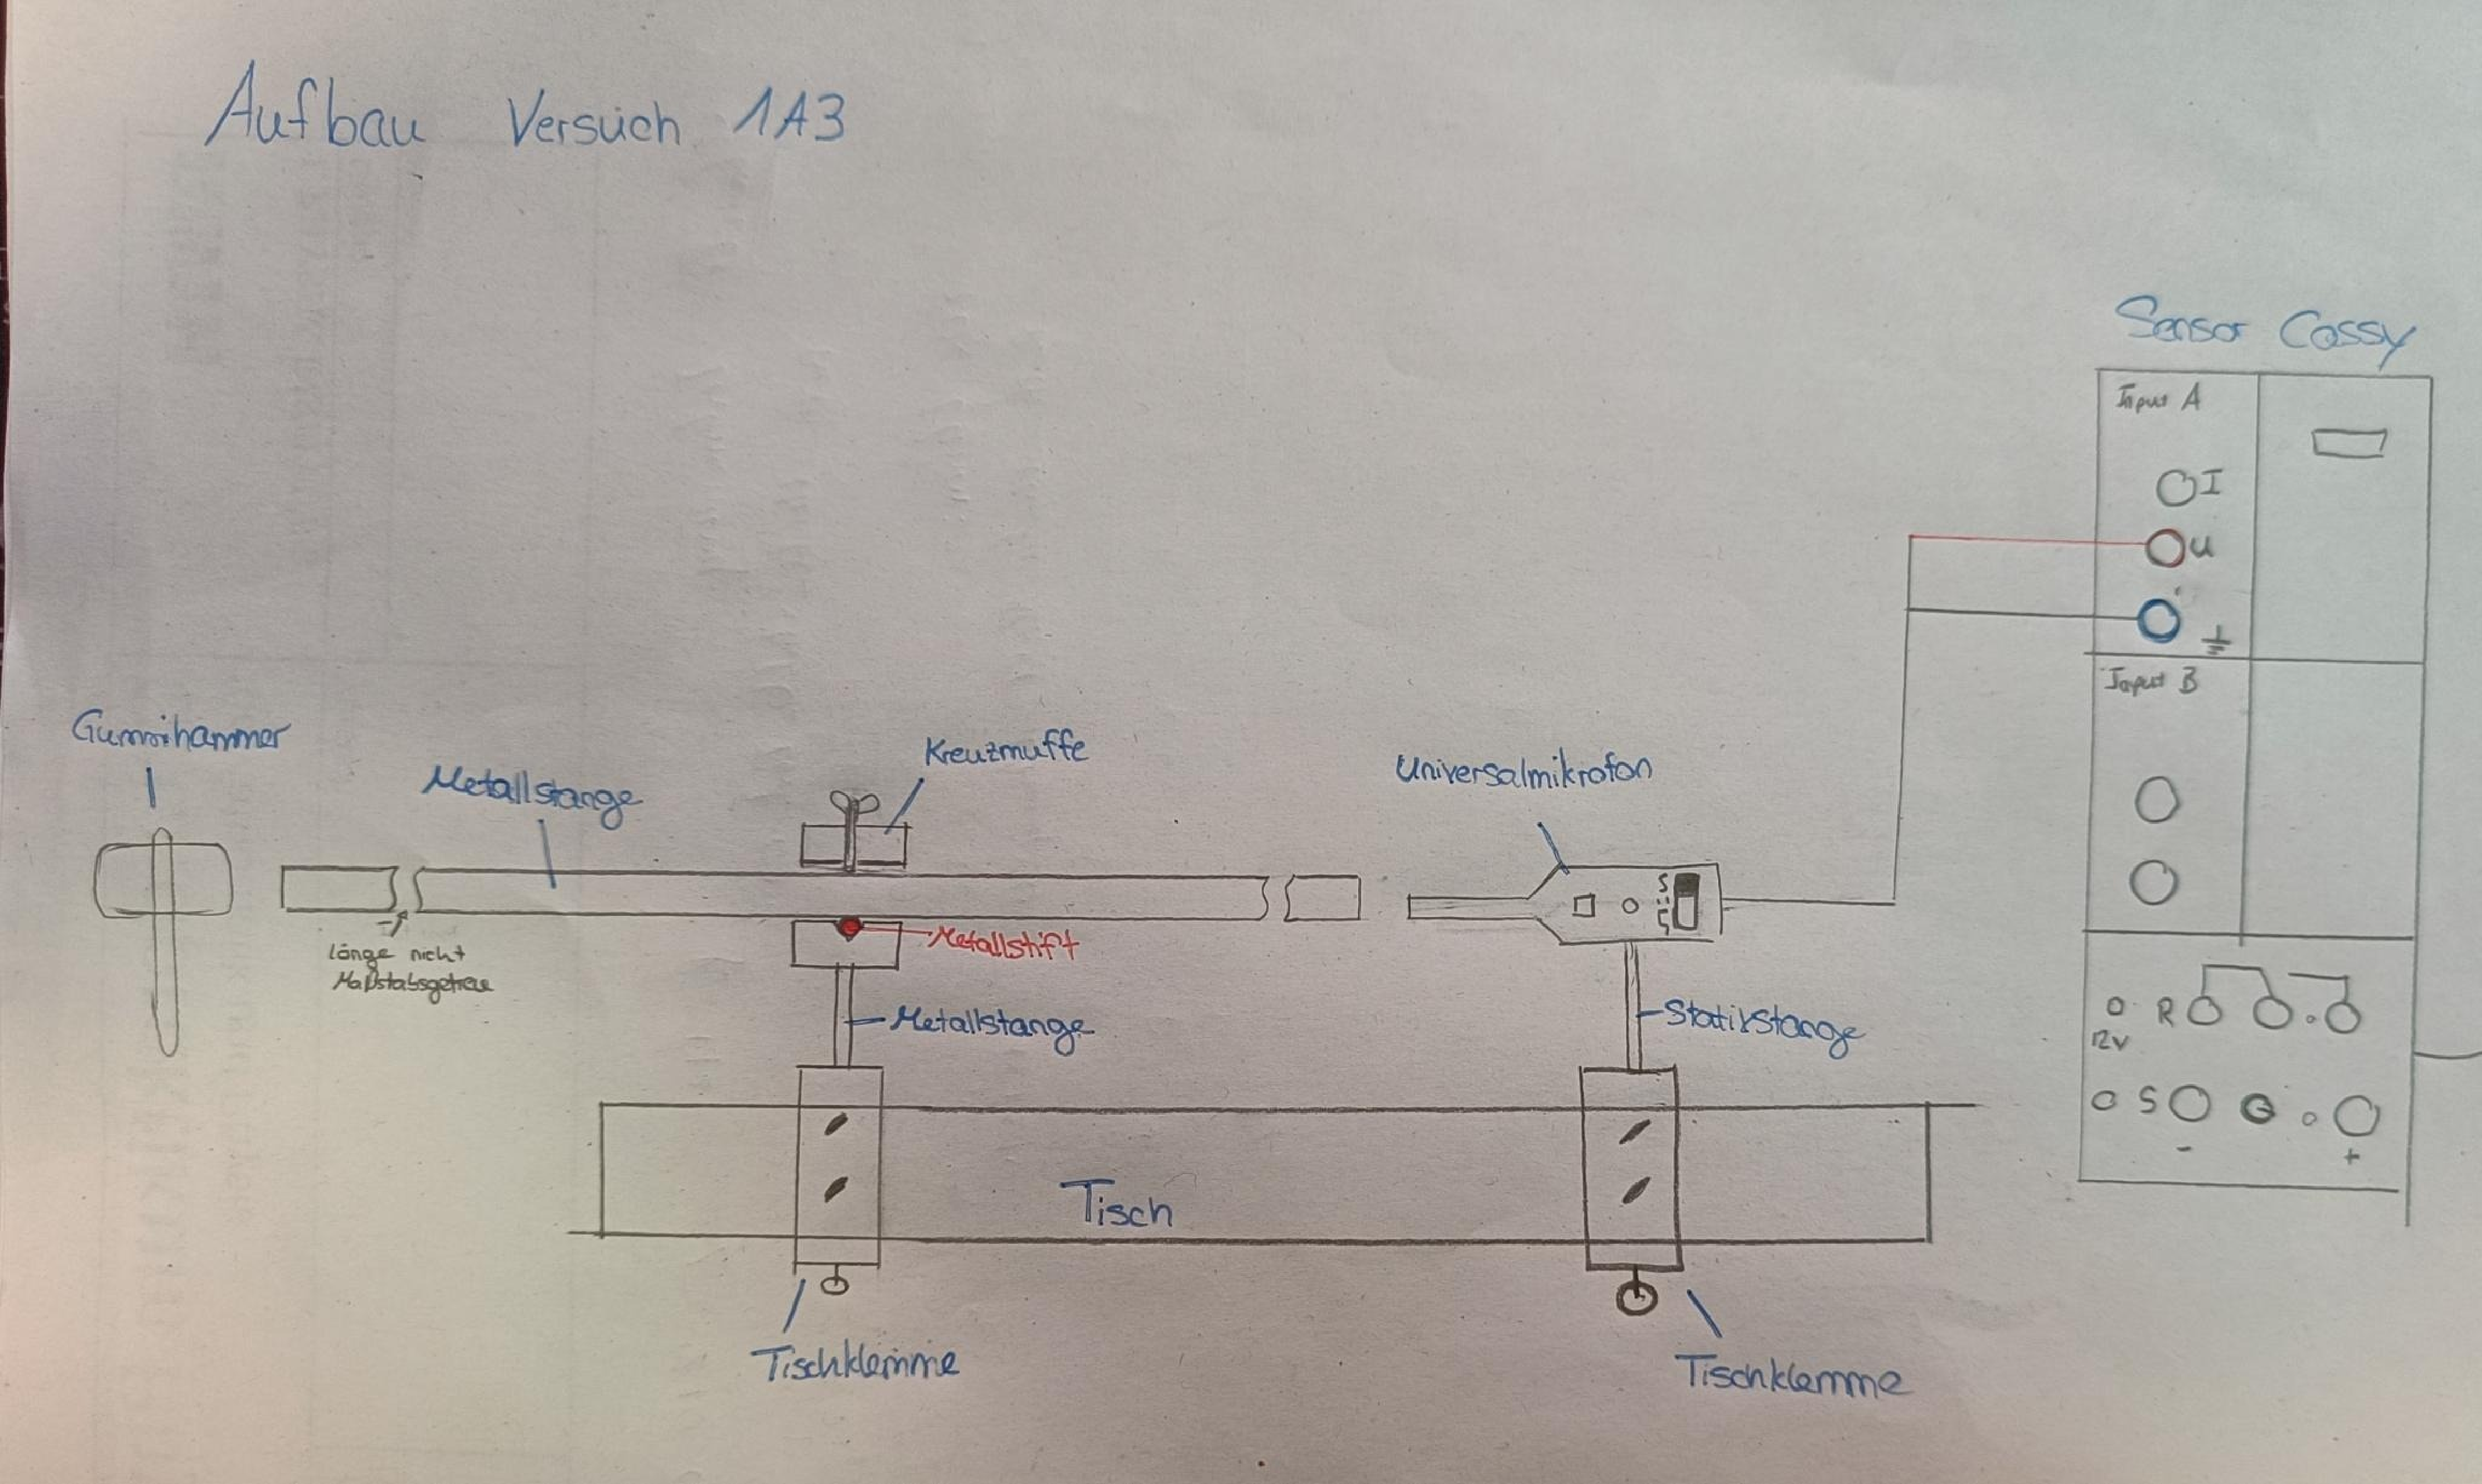
\includegraphics[width=1\textwidth]{Bilder/434170_428396_1A3_SkizzeAufbau.pdf}
  \caption{Skizze des Versuchsaufbaus}
  \centering
\end{figure}
 
Der Aufbau des Experiments kann der oben stehenden Skizze entnommen werden. 

Zunächst werden mit zwei Tischklemmen Mikrofon und Metallstange an dem Tisch befestigt. Wobei die Stange mithilfe der Kreuzmuffe befestigt wird. In die Kreuzmuffe wird der Metallstift ortogonal zu der Stange hineingelegt, sodass diese beim mittigen einspannen nur an einem Punkt unterstütz wird. Die Stange also frei schwingen kann. 

Das Universalmikrofon und die Metallstange werden auf eine Linie gebracht, mit 5mm Abstand. Sodass Das Mikrofon die Schallwellen gut aufzeichnen kann, aber nicht beschädigt wird, falls die Stange zu stark angeschlagen wird. Wärend der gesamten durchführung muss darauf geachtet werden, dass die Position der beiden sich nicht gegeneinander verschieben. 


Das Universalmikrofon wird in den Sensor CASSY eingesteckt, wobei das Gelbe Kabel(in der Skizze rot) in die Buxe für die Spannung, und das schwarze in die für die Erdung gesteckt wird. Das Mikrofon wird auf den Amplitudenmodus $\sim$ gestellt. Der Gummihammer wird verwendet um auf das, dem Mikrofon abgewandte, Ende der Metallstange zu schlagen. Damit werden die Metallstangen zum schwingen angeregt.

\subsection{Durchführung}

Zunächst haben wir die Metallstangen kategorisiert nach dem Material aus welchem sie bestehen.

\begin{itemize}
\item Aluminium:		 matt silberne Stange 
\item Messing:		 goldene Stange
\item Kuper:			 kupferfarbene Stange
\item Stahl 15:		 silber glänzende Stange
\end{itemize}

Von diesen haben wir dann jewails, Länge, Masse und Durchmesser bestimmt. 
Die Länge haben wir mit dem Bandmaß gemessen, wobei hier darauf geachtet wurde, dass das Bandmaß straff ist. Die Masse haben wir mit der Analysewage bestimmt, indem wir die Stange mittig auf der Wage plaziert haben. 


Da wir bei der Stange annehmen, dass diese einen kreisförmigen querschnitt hat, was nicht perfekt zutreffen wird, führen wir die Messung des Durchmessers mehrfach durch. Hierfür verwenden wir die Mikrometerschraube. Wir messen an verschiedenen Stellen, dabei rotieren wir die Stange beliebig bei jeder Messung um die längsachse. Dies wiederholen wir zehn mal. Sodass wir für jede Stange 10 Messwerte für den Durchmesser haben.\\ 

\begin{figure}[H]
  \centering
  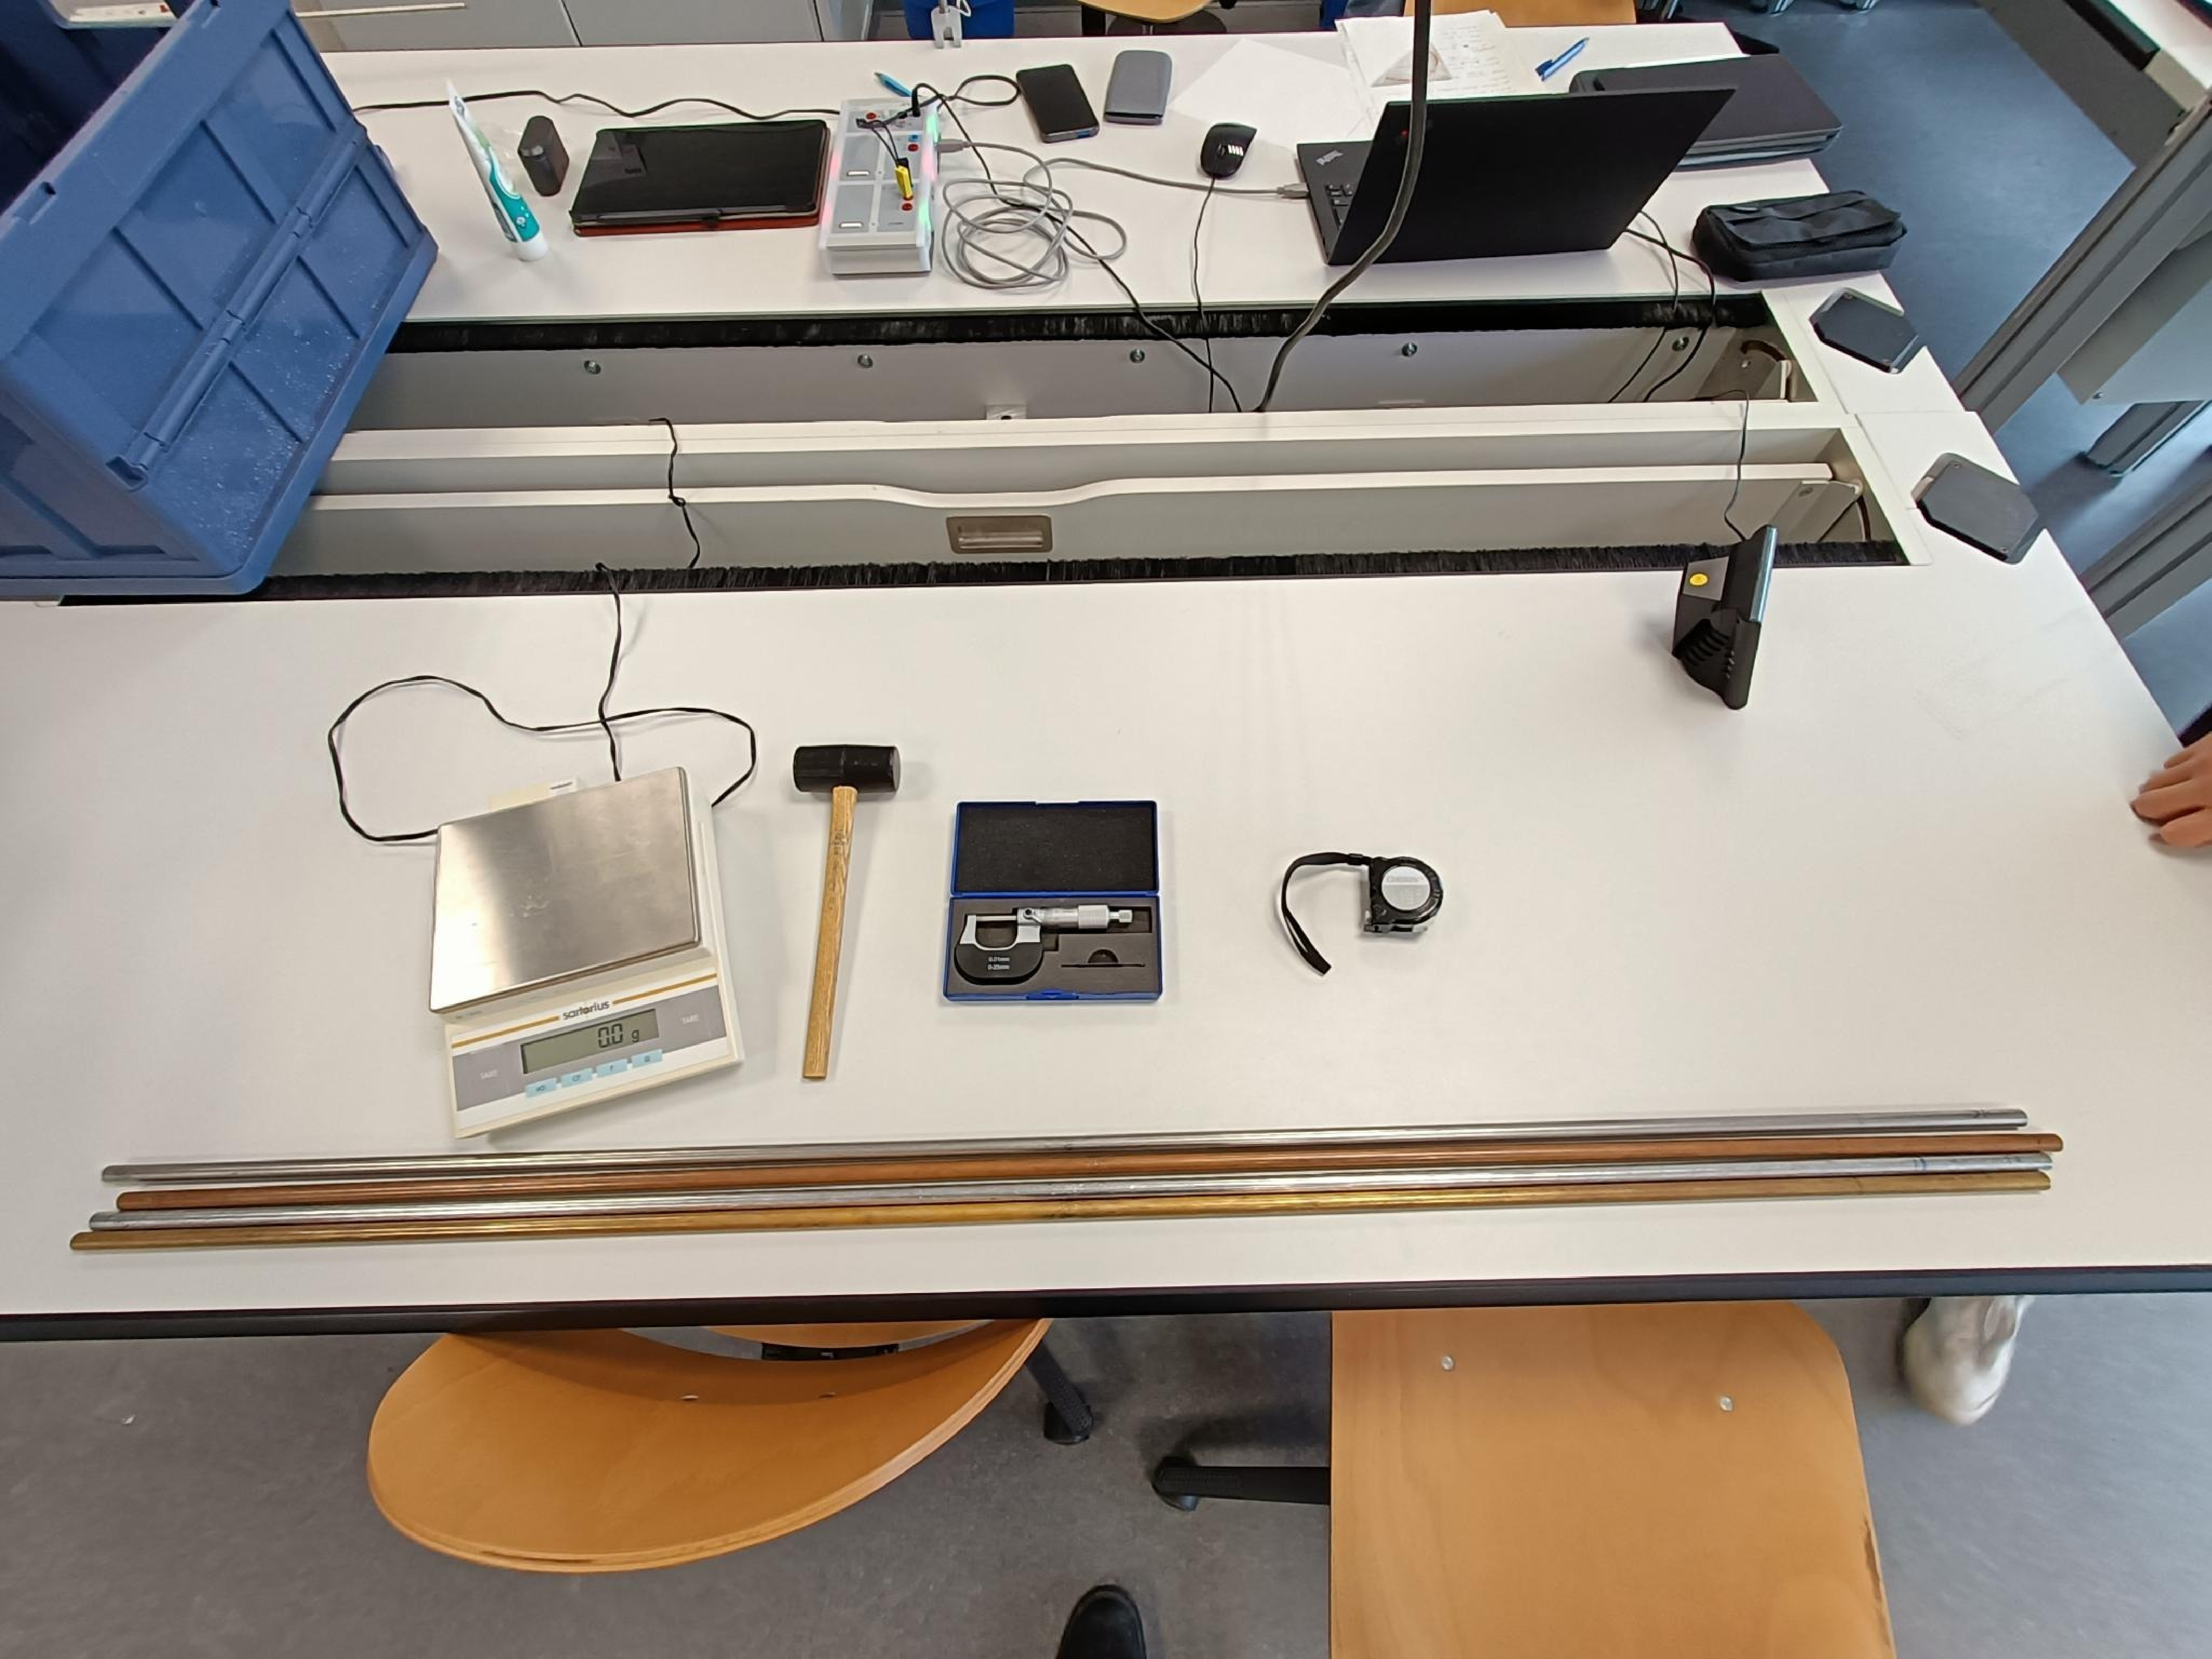
\includegraphics[width=0.8\textwidth]{Bilder/434170_428396_1A3_Materialien.pdf}
  \caption{Bild der Messgeräte und Metallstangen}
  \centering
\end{figure}

Als nächstes bauen wir den Versuch auf. Hier gehen wir genau so vor wie in der vorherigen beschreibung des Versuchsaufbaus. Als erstes haben wir die Kupferstange verwendet.
Wobei wir zunächst die Tischklemme plaziert haben und die Stange mittig eingespannt. Hierfür haben wir von einem Ende der Stange auß, mit dem Maßband die Mitte bestimmt. Dann haben wir das Mikrofon passend zu der Stange positioniert, und an den Tisch montiert. Hierbei haben wir noch beachtet, dass die Stange nicht zu fest eingespannt werden sollte, da dies auswirkung auf die Frequenz hat. Außerdem haben wir überprüft, dass sie nur an einem Punkt aufliegt, sodass sie frei schwingen kann. Die Spitze des Mikrofons haben wir ungefähr 5mm entfernt vom Ende der Stange positioniert. Dies haben wir nach Augenmaß getan. 

\begin{figure}[H]
  \centering
  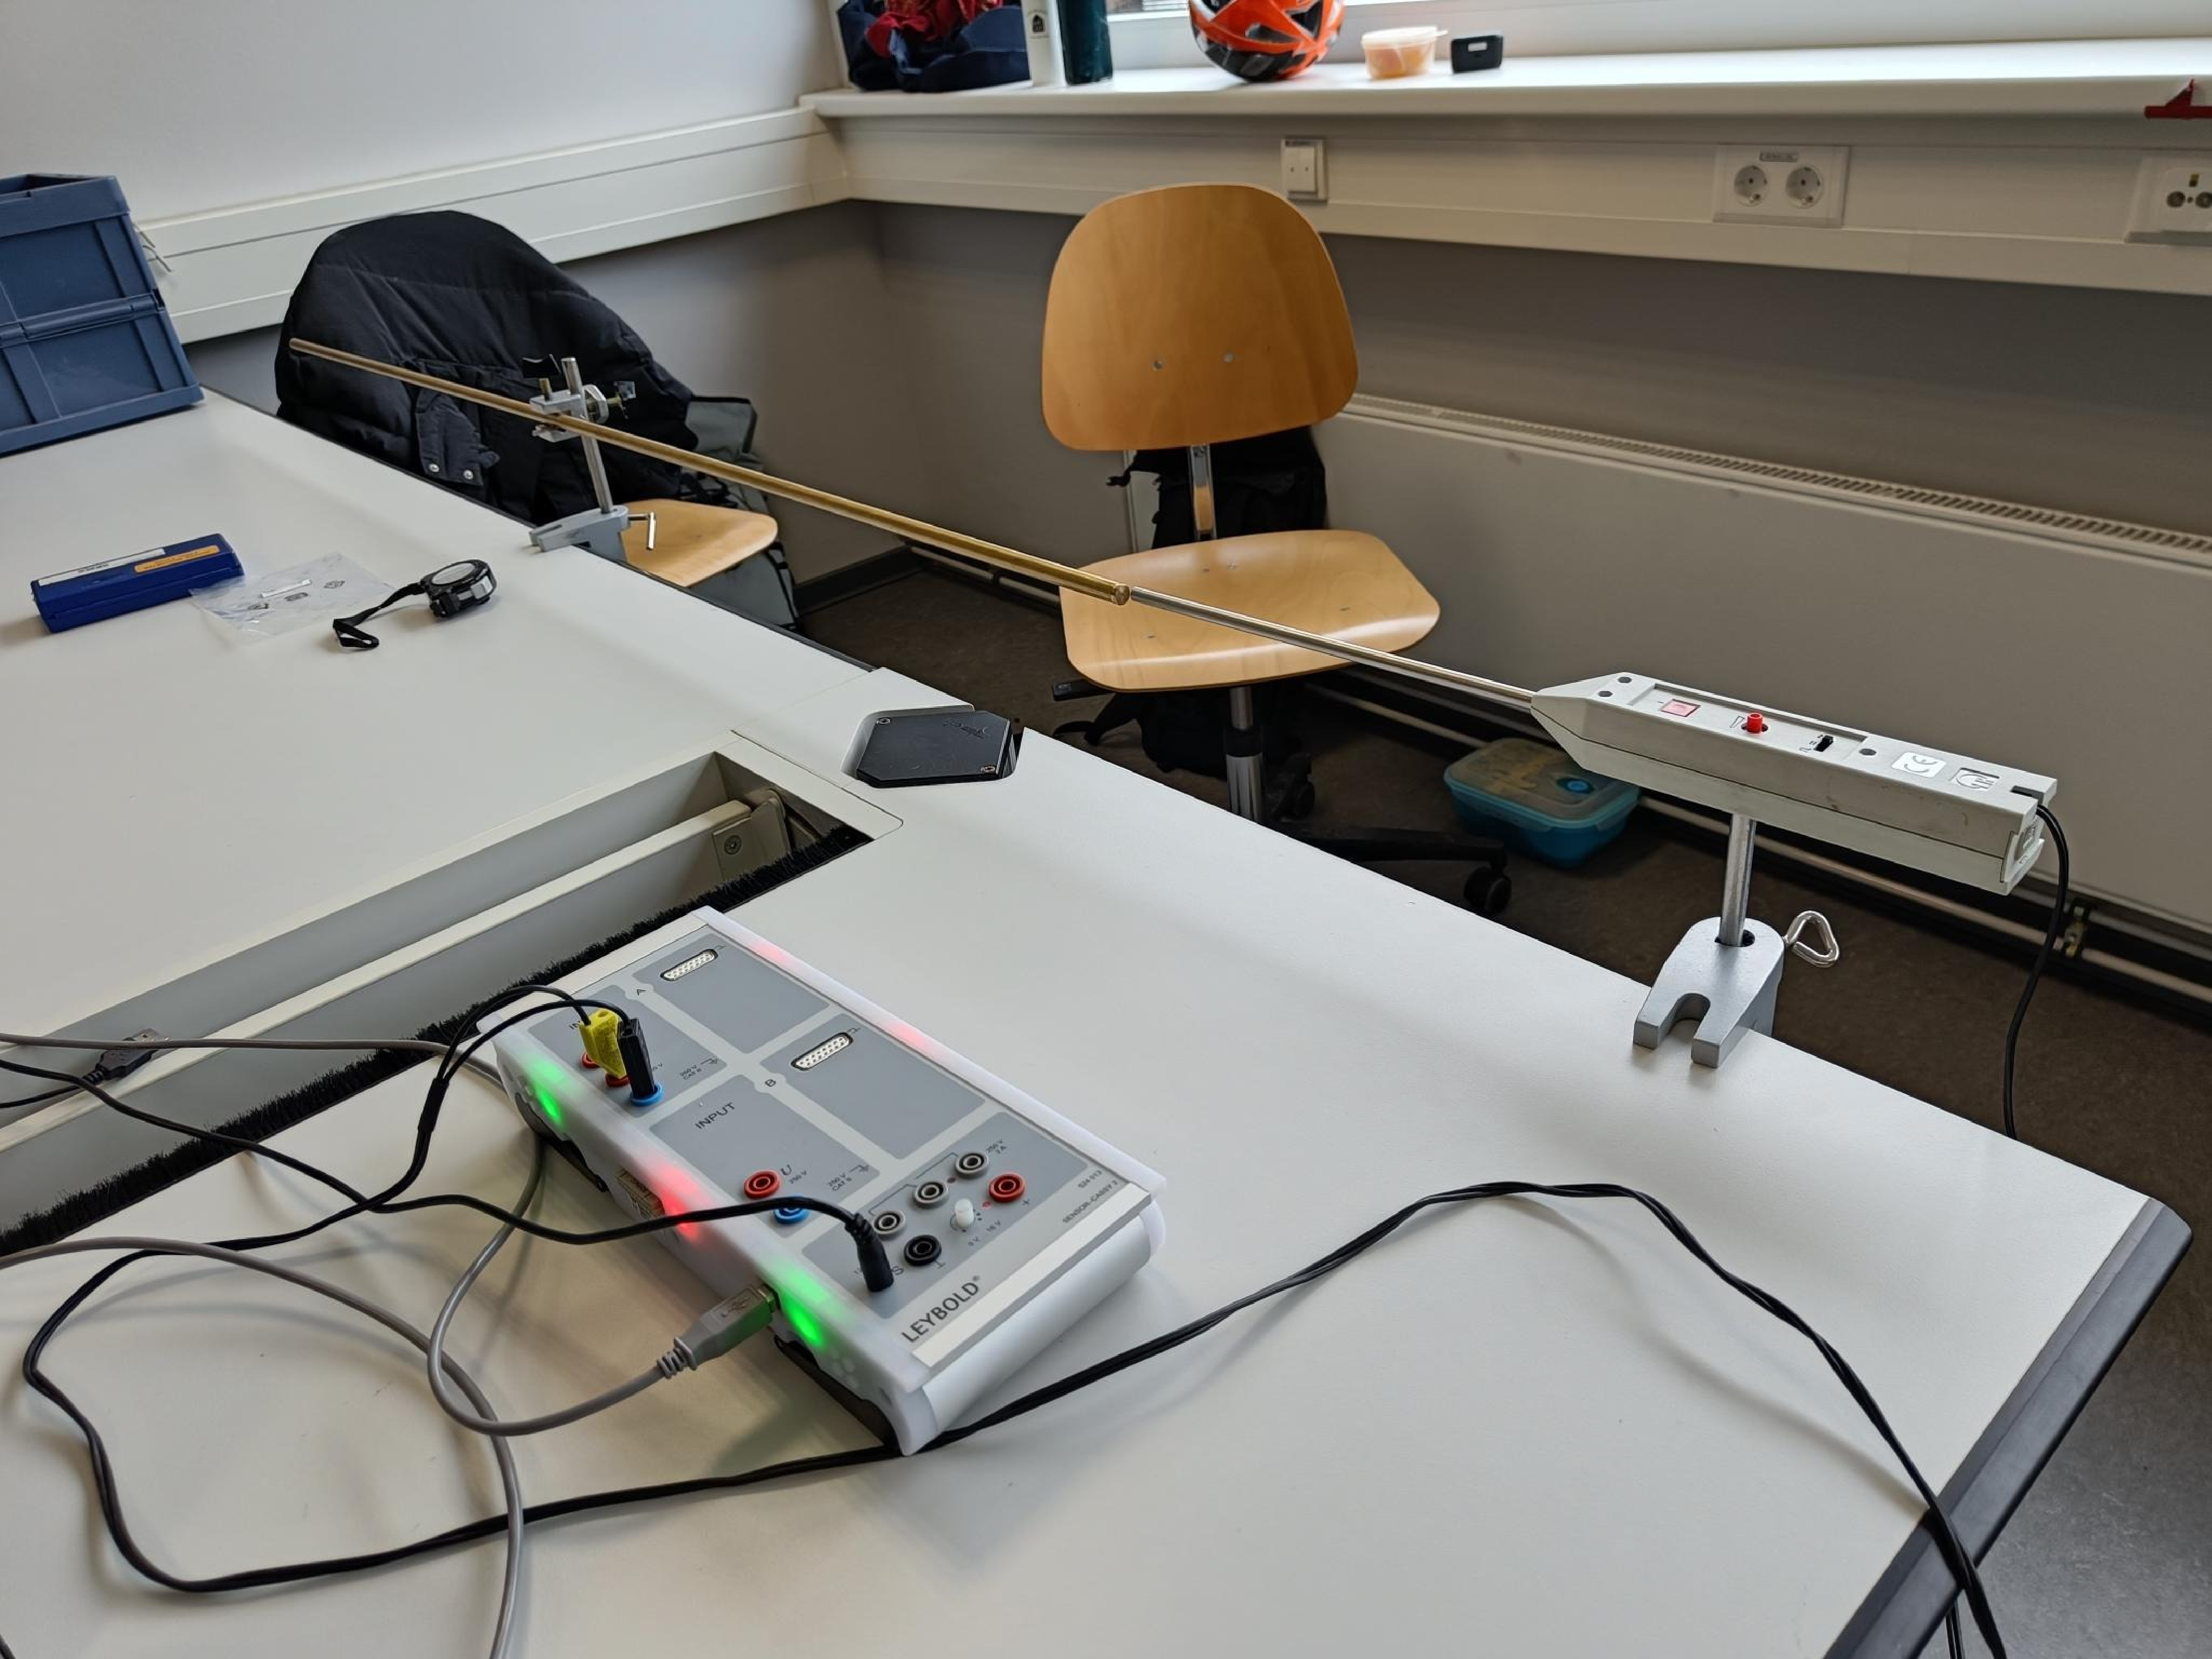
\includegraphics[width=0.8\textwidth]{Bilder/434170_428396_1A3_Gesamtaufbau.pdf}
  \caption{Bild der fertig aufgebauten Versuchsanordnung}
  \centering
\end{figure}

Dann haben wir das Mikrofon wie im Aufbau beschrieben an das Sensor Cassy angeschlossen und in betrieb genommen. Zunächst haben wir uns überlegt, was sinnvolle Messparameter sind. Da die Schallgeschwindigkeit in Metallen im bereich von mehrere 1000m/s liegt, muss das Messintervall im bereich von 10-100$\mu$s sein. Somit haben wir erste Testmessungen durchgeführt. Wobei wier diese mehrfach wiederholt haben, bis wir die Empfindlichkeit des Mikrofons so eingestellt hatten, dass wir den gesamten dynamischen bereich des Mikrofons ausnutzen, und nicht in die Sättigung kommen. Dann konnten wir eine erste FFT mit CASSY durchführen, und mit peakfinder die Frequenz des schwingenden Kupferstabs ungefähr bestimmen. Mit diesen Informationen haben wir dann unsere Messparameter eingestellt.\\

\textbf{Messparameter:}
\begin{itemize}
\item Messzeit: 3s
\item Intervall: 100$\mu$s
\item Anzahl Messungen: 30001
\item Spannungsbereich: -3V bis 3V (Da der dynamisch Bereich des Mikrofons 2.5V ist)
\end{itemize}

Wir haben für die Messung keinen Trigger verwendet, sondern die Messung manuell gestartet. 


Bei einer Messung hat einer aus unserer Gruppe mit dem Gummihammer den Kupferstab angeschlagen, wärend die andere Person kurz nach Anschlag die Messung gestartet hat, so dass, der Einschwingvorgang möglichst nicht mit aufgezeichnet wurde. Wir haben versucht den stab immer möglichst gleich an zu schlagen, also gleiche position und Kraft, damit die Messungen möglichst vergleichbar sind. Außerdem haben wir darauf geachtet, dass wir die Stange nur dann anschlagen, wenn niemand anders eine Stange des gleichen Materials anschlug.

\begin{figure}[H]
  \centering
  \subfloat[Anschlagen der Stange]{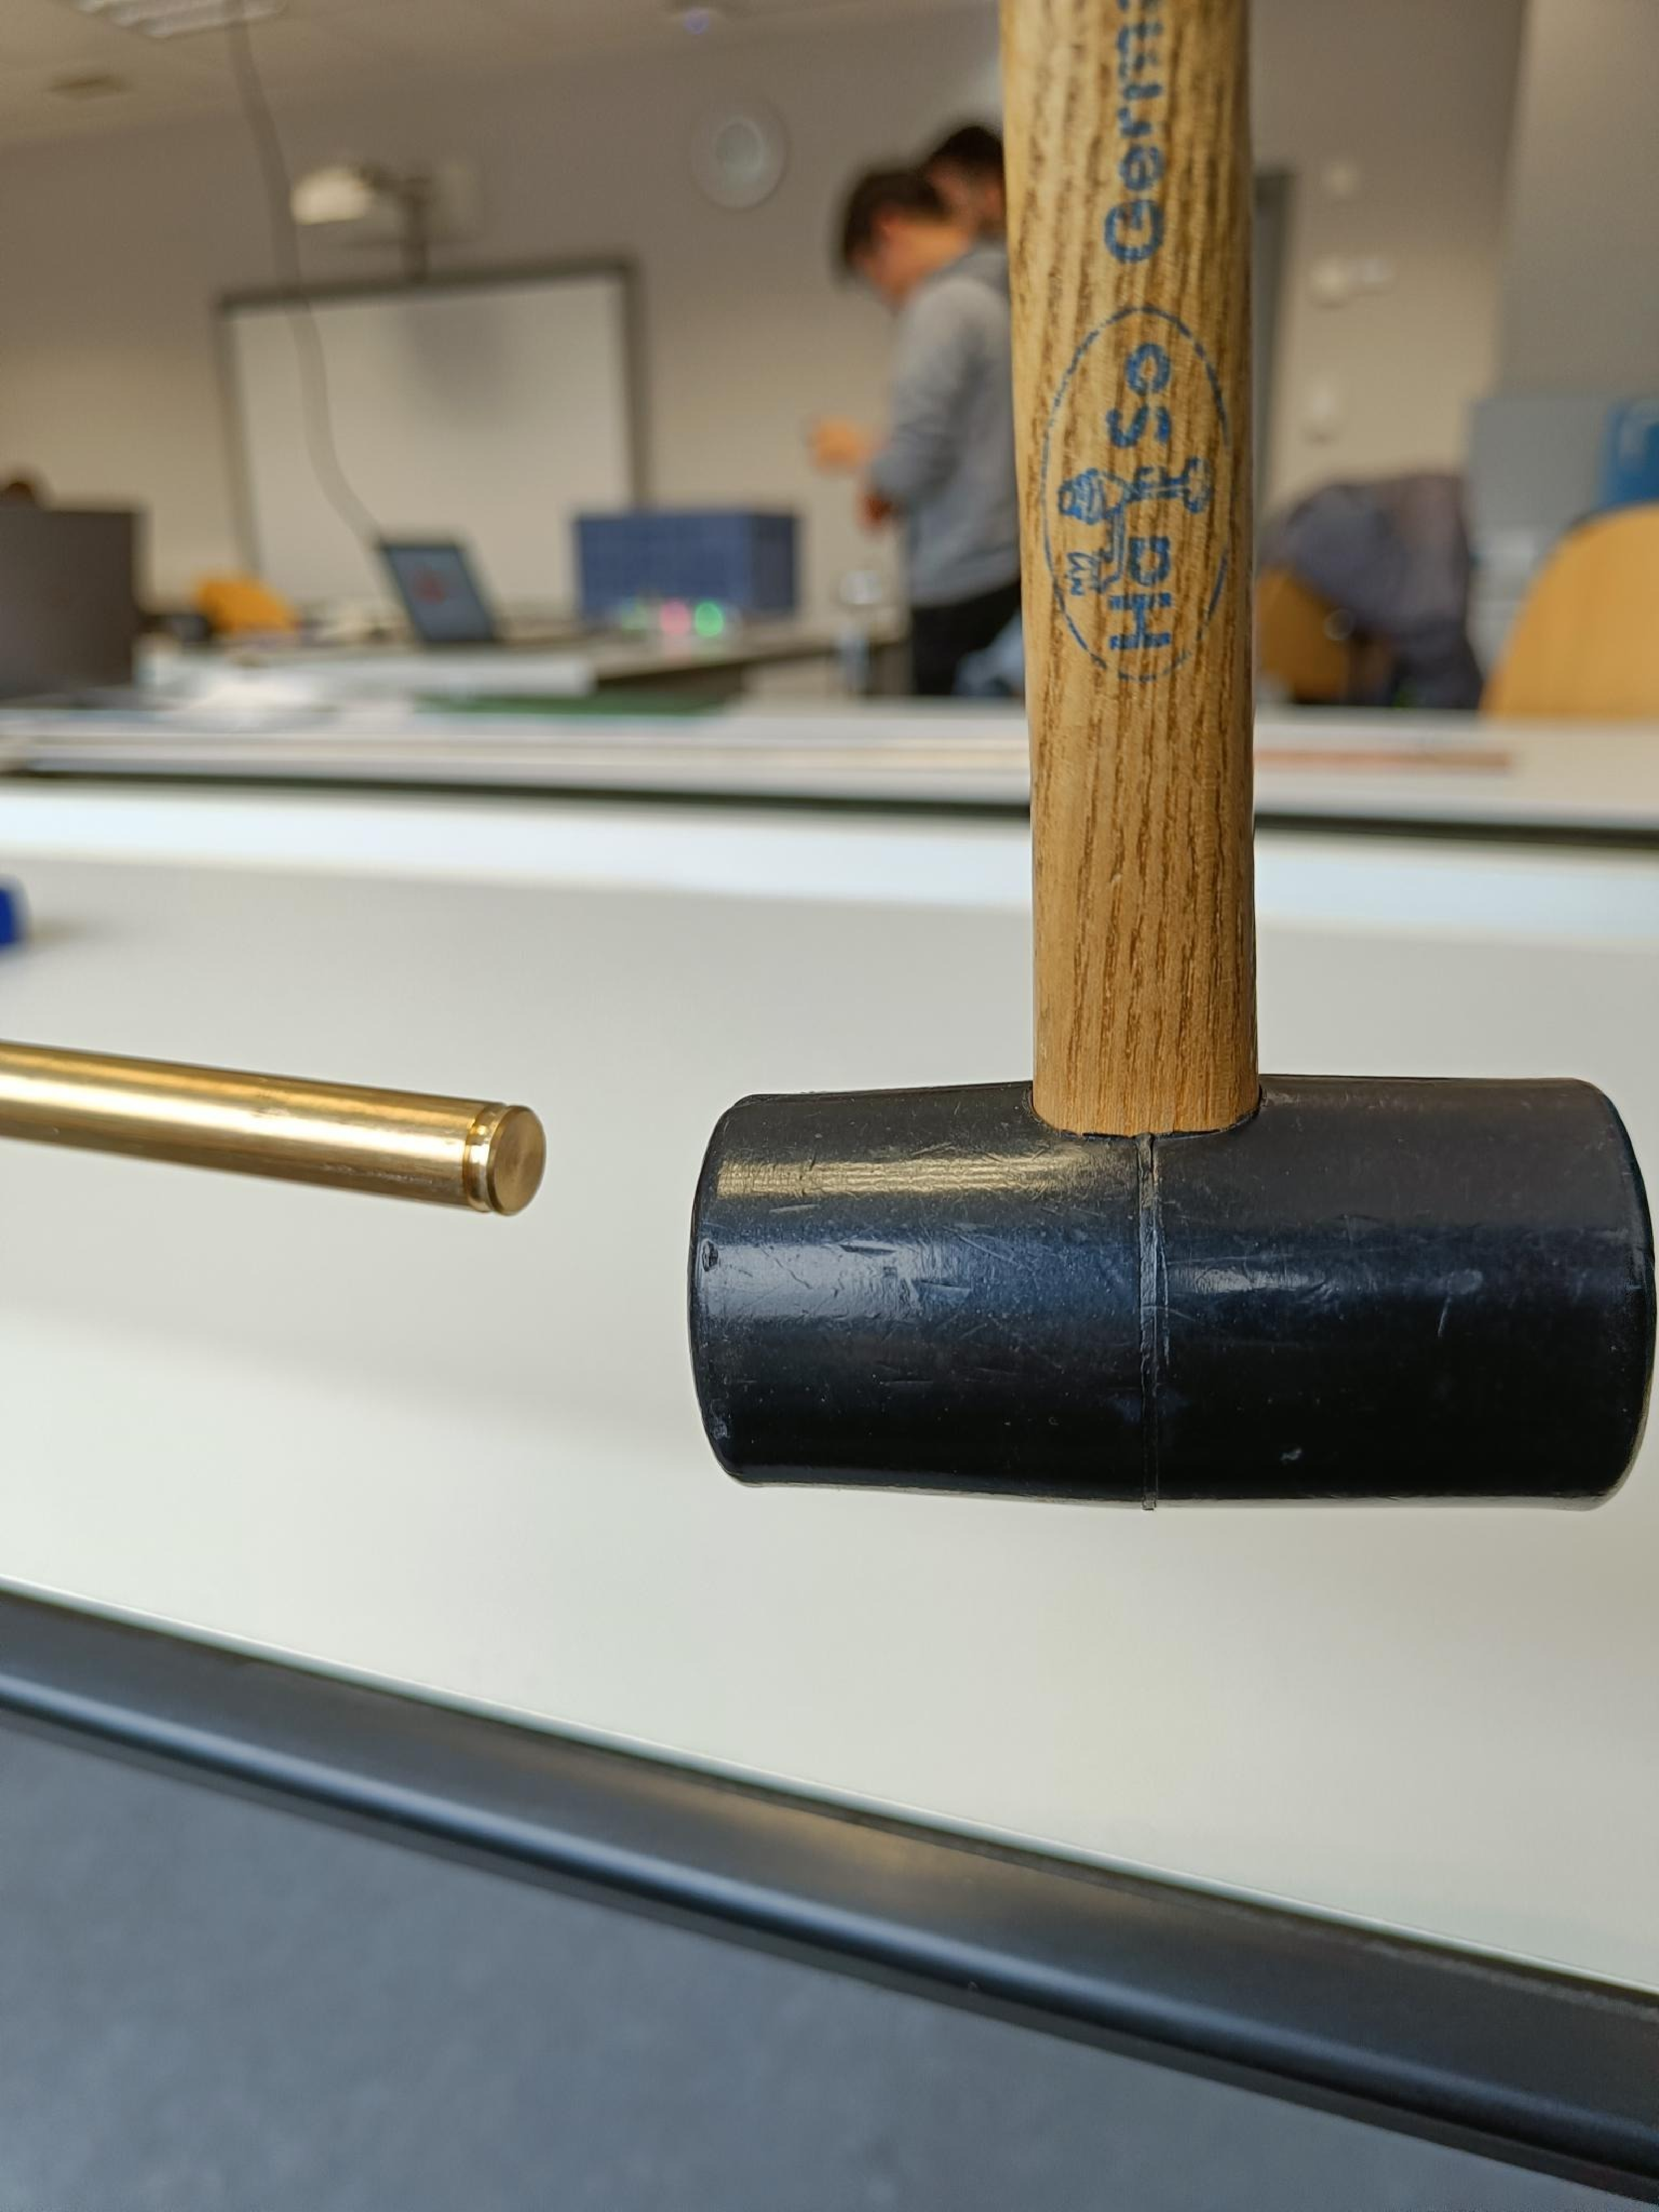
\includegraphics[width=0.3\textwidth]{Bilder/434170_428396_1A3_Hammer.pdf}\label{fig:f1}}
  \hfill
  \subfloat[Position von Stange und Mikrofon]{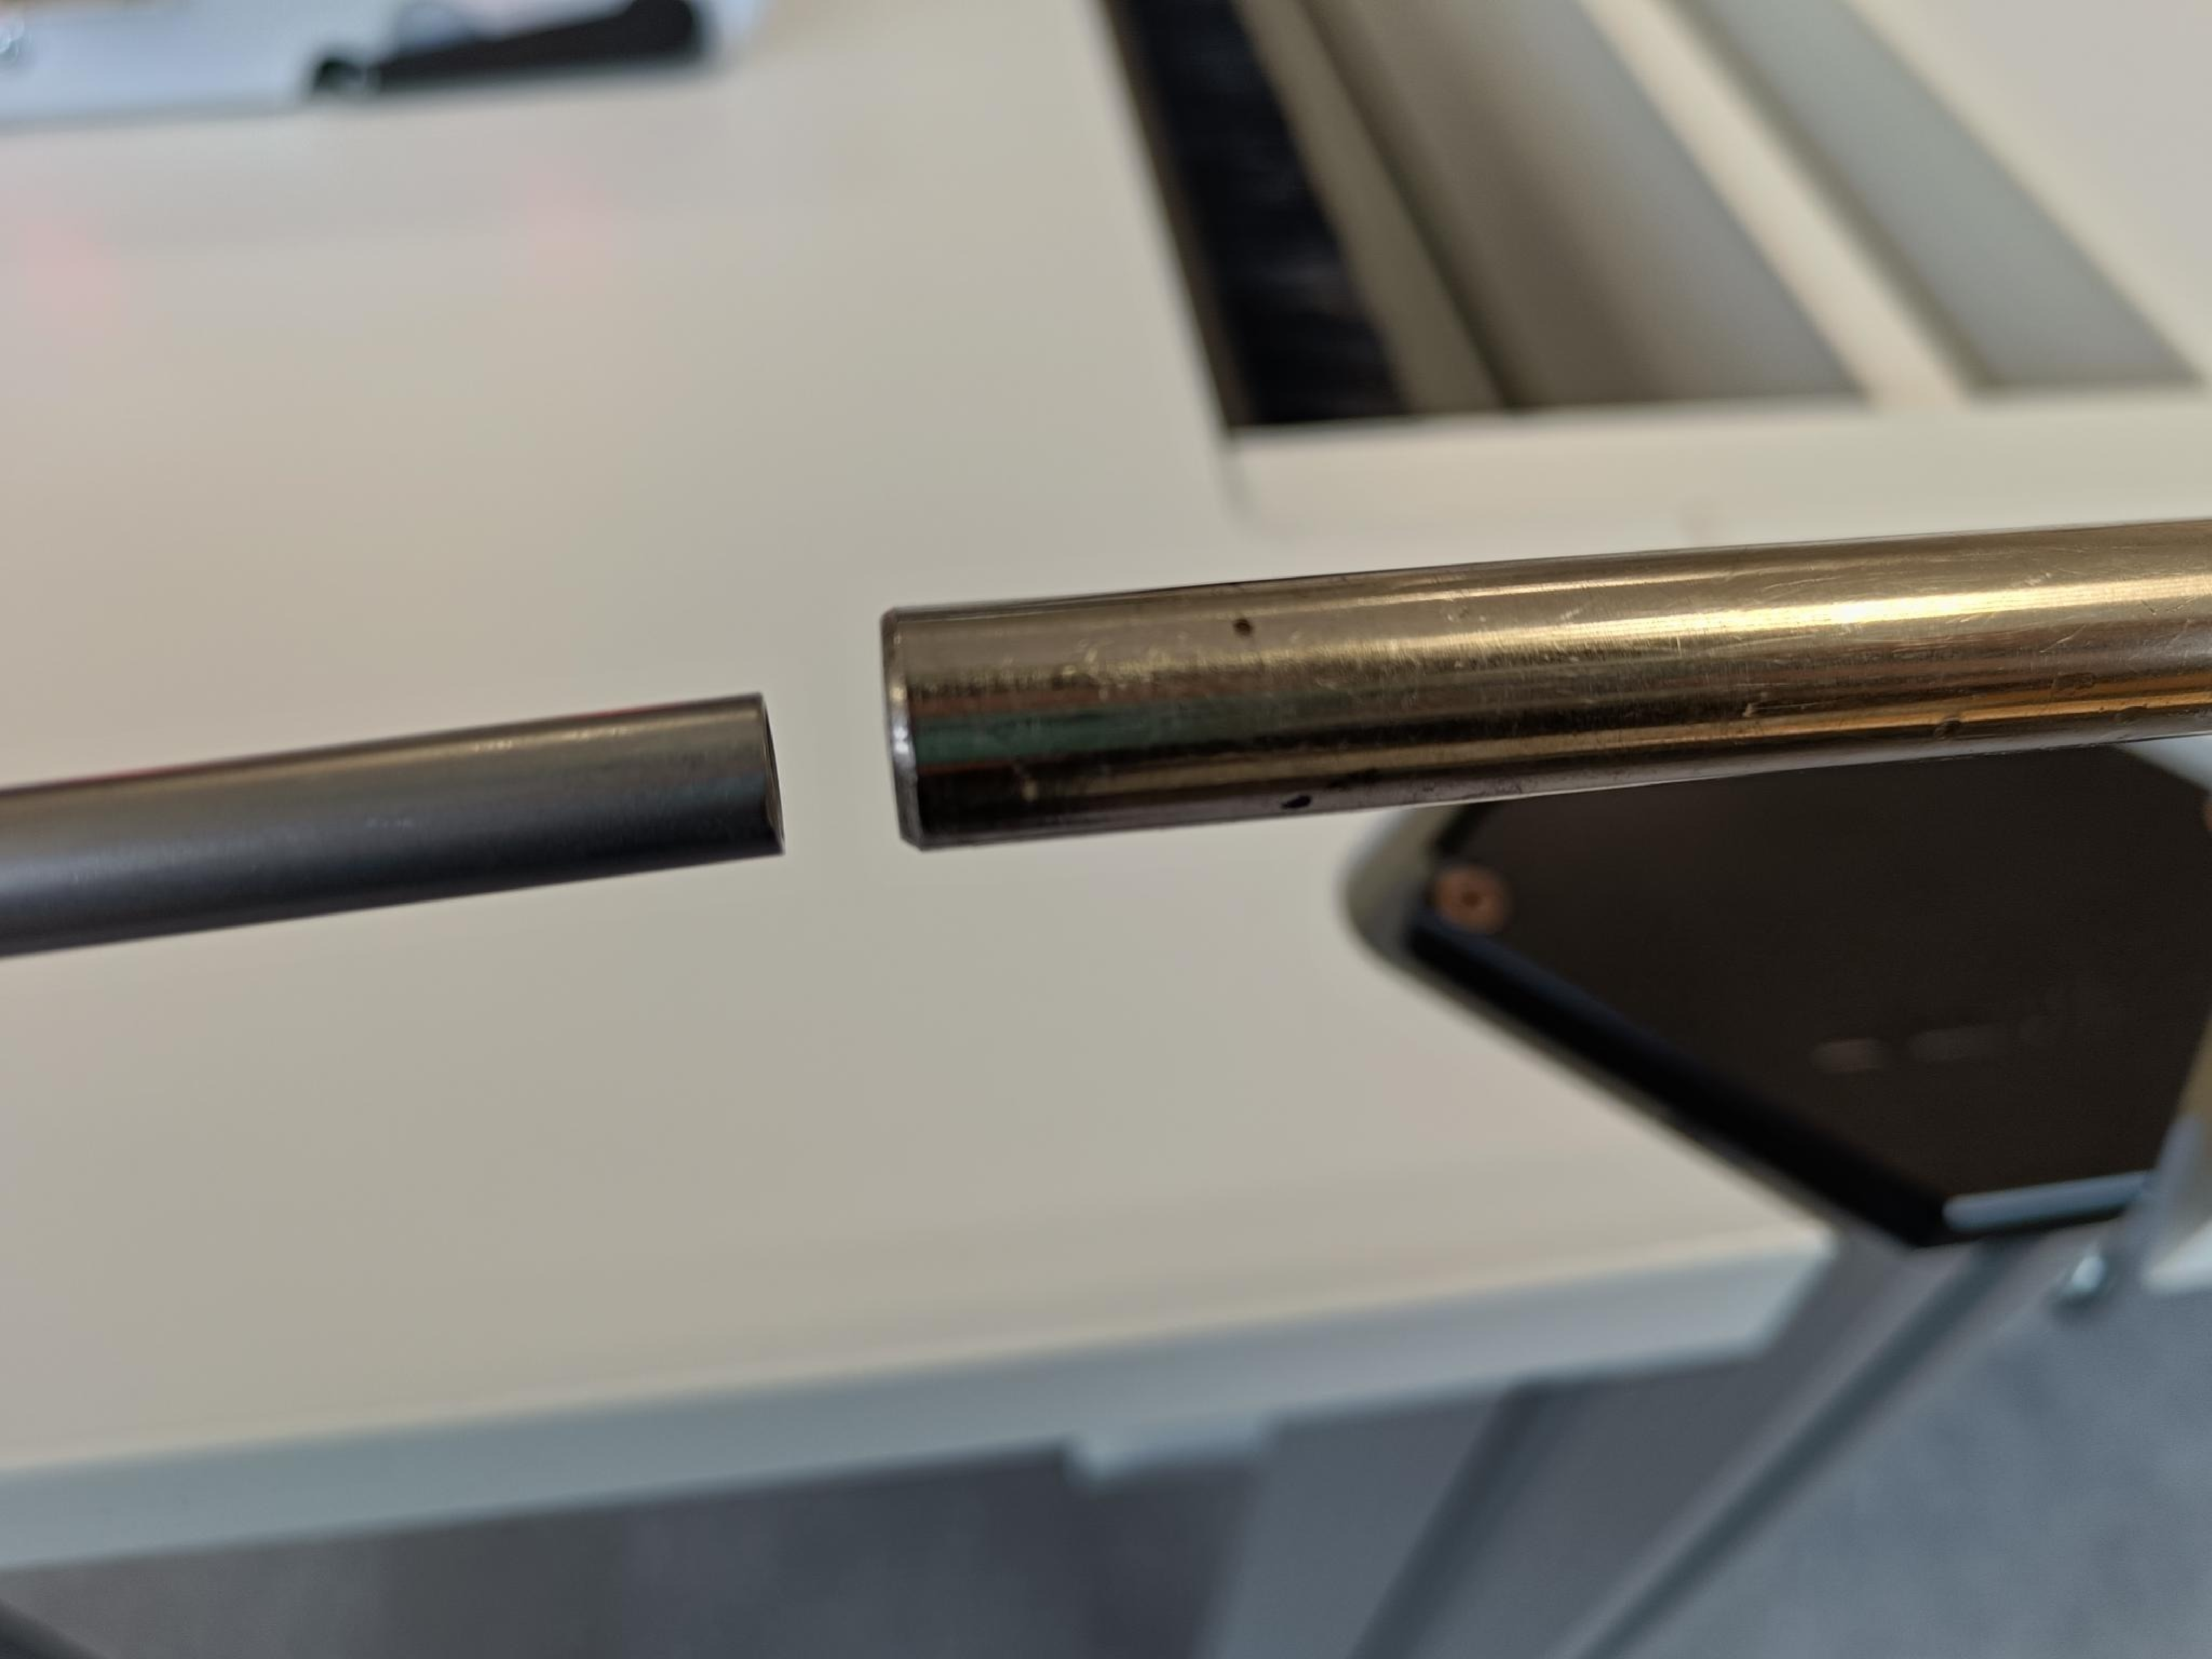
\includegraphics[width=0.5\textwidth]{Bilder/434170_428396_1A3_MSNahaufnahme.pdf}\label{fig:f2}}
  \caption{Anordnung zur Durchführung einer Messung}
\end{figure}



Mit unseren eingestellten Messparametern haben wir dann eine erste vollständige Testmessung durchgeführt um zu überprüfen, ob alle Einstellungen gut passen. Aus dieser Messung haben wir erneut mit der FFT die Frequenz der Grundschwingung bestimmt. Mit dieser konnten wir eine erste Überschlagsrechnung für das E-Modul von Kupfer anstellen.
Diese ist im Messprotokoll zu finden. Da der Wert in der erwarteten Größenordnung lag, haben wir die Messreihe mit diesem Aufbau gestartet. 


Insgesamt haben wiir die Messung gleich wie bei der Testmessung 10 mal durchgeführt, und die Ergebnisse mithlife der FFT des CASSY Lab 2 grob auf konsistenz überprüft. Diese Messungen haben wir als unsere Messreihe abgespeichert.\\

Die Frequenz ist auch abhängig von der Einspannung der Stange, also von der Kraft und der position und der orientierung der Einspannung. Weswegen der Fehler aufgrund dieser Effekte auch beachtet werden muss. Dazu haben wir mit der Kupferstange Messungen durchgeführt bei denen wir die Einspannung um 1cm-2cm um den mittelpunkt variiert haben, sowie die Kraft mit der sie eingespannt ist, als auch die Rotation um die Längsachse.
Diese haben wir als Messreihe für spätere bestimmung des Fehlers gespeichert.\\

\begin{figure}[H]
  \centering
  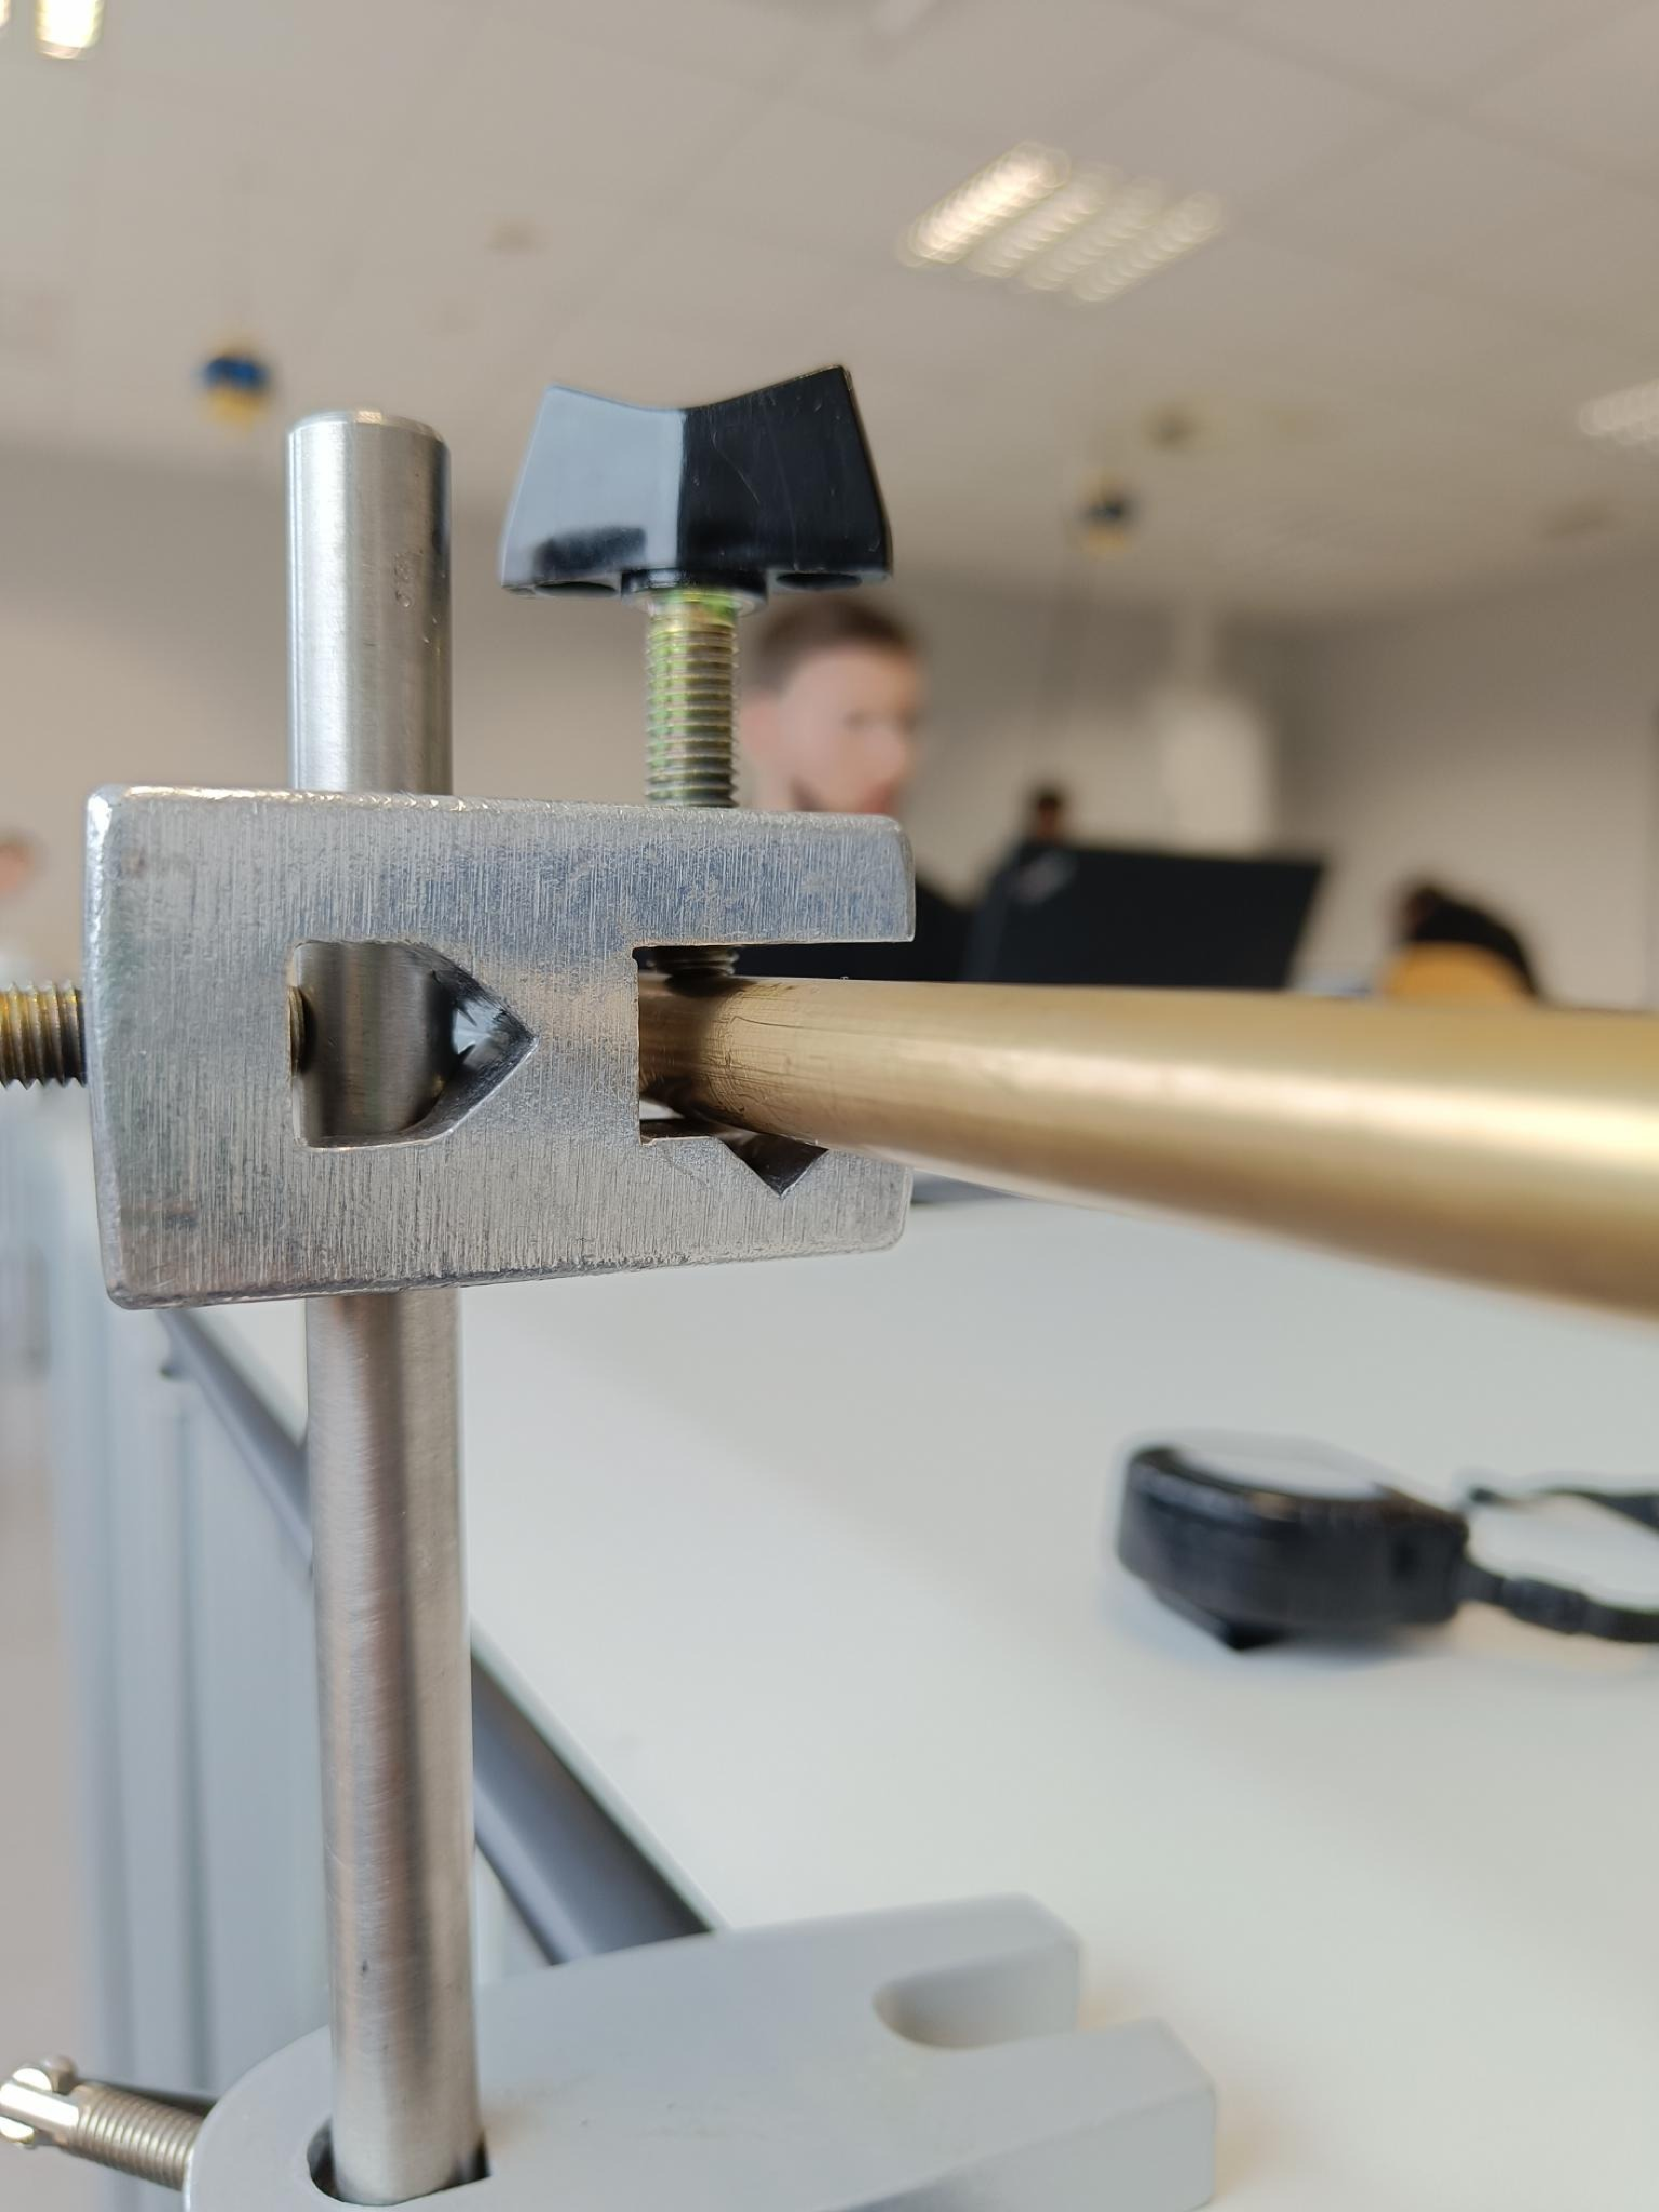
\includegraphics[width=0.8\textwidth]{Bilder/434170_428396_1A3_Einspannung2.pdf}
  \caption{Einspannungspunkt der Stange}
  \centering
\end{figure}

Das selbe Vorgehen wie bei der Kupferstange haben wir auch bei den anderen Stangen durchgeführt. Wobei wir jedes mal zunächst eine Testmessung gemacht habe, um die Empfinlichkeit des Mikrofons für das Material spezifisch ein zu stellen, und zu sehen ob die gemessene Frequenz, und damit auch das E-Modul den Erwartungen entspircht. 

Sämtliche gemessenen Daten haben wir gespeichert, sodass wir diese zur Auswertung verwenden können. einige Messungen mussten wir wiederholen, da wir die Stange nicht richtig angeschlagen hatten, oder sie sich beim Anschlag vom Mikrofon weggedreht hat. Ach durch Störgeräusche anderer Stangen, oder lautes Reden wurden einige Messungen gestört weswegen wir sie erneut durchführten.\\

Nach beendigung aller Messungen haben wir alles wieder abgebaut und an die dafür vorgesehenen Orte zurrückgelegt. 


\end{aufgabe}

\begin{aufgabe}{Rohdaten}

Der untenstehenden Tabelle können die Masse und die Länge der vermessenen Metallstangen entnehmen.  
    \begin{table}[H]
        \centering
        \begin{tabularx}{0.8\textwidth}{X c c} % adjust width as needed
            \toprule
            \textbf{Metall Stange} & \textbf{Masse} & \textbf{Länge} \\
            \midrule
            Aluminium & 460.9g & 150cm \\
            Messing & 1427.5g & 150cm \\
            Kupfer & 1505.4g & 150cm \\
            Stahl 15 & 1327.4g & 150cm \\
            \bottomrule
        \end{tabularx}
        \label{tab:mytable}
    \end{table}

In dieser Tabelle finden sie die Messung des Durchmessers. Diese haben wir pro Stange 10 mal durchgeführt. Gemessen wurde mit der Milimeterschraube an verschiedenen Positionen.
    \begin{table}[H]
        \centering
        \begin{tabularx}{0.8\textwidth}{X c c c c} % adjust width as needed
            \toprule
            \textbf{Messung} & \textbf{Aluminium} & \textbf{Messing} & \textbf{Kuper} & \textbf{Stahl 15} \\
            \midrule
            1. & 12.05mm & 11.98mm & 11.98mm & 12.00mm \\
            2. & 12.05mm & 12.01mm & 11.98mm & 12.00mm \\
            3. & 12.06mm & 11.98mm & 11.98mm & 11.99mm \\
            4. & 12.05mm & 11.99mm & 11.98mm & 12.00mm \\
            5. & 12.06mm & 11.98mm & 11.98mm & 12.00mm \\
            6. & 12.06mm & 11.98mm & 11.98mm & 12.00mm \\
            7. & 12.06mm & 11.99mm & 11.98mm & 12.00mm \\
            8. & 12.05mm & 11.99mm & 11.98mm & 12.00mm \\
            9. & 12.06mm & 11.98mm & 11.98mm & 12.00mm \\
            10.& 12.07mm & 11.98mm & 11.98mm & 12.01mm \\
            \bottomrule
        \end{tabularx}
        \label{tab:mytable}
    \end{table}

Im Verlauf der Durchführung des Versuches haben wir verschiedene Messreihen aufgenommen. Wobei wir für jeden Stabe eine Reihe von 10 Messungen durchgeführt haben. Bei dem Kupferstab haben wir noch eine Messreihe aufgenommen, die wir später verwenden werden um den Systematischen Fehler aufgrund der Einspannung zu bestimmen. Zur übersichtlichkeit und damit im Späteren Verlauf klar ist Welche Messreihe welche ist, hier noch eine Auflistung von diesen:\\

    \begin{table}[H]
        \centering
        \begin{tabularx}{1\textwidth}{c X X} 
            \toprule
            \textbf{Messreihe} & \textbf{Name} & \textbf{Beschreibung} \\
            \midrule
            1. & Kupfer\_Messung & 10mal Messung der Schwingung der Kupferstange \\\\
            2. & Alu\_Messung & 10mal Messung der Schwingung der Aluminiumstange \\\\
            3. & Stahl\_Messung & 10mal Messung der Schwingung der Stahlstange \\\\
            4. & Messing\_Messung & 10mal Messung der Schwingung der Messingstange \\\\
            5. & Kupfer\_Einsp\_Fehler & 6mal Messung der Schwingung bei verschiedenen 				Einspannpositionen Orientierungen und Kraft.  \\\\  
            6. & Material\_Test & Pro Material einmalige Testmessung, zur überprüfung das alle Parameter stimmen \\
            \bottomrule
        \end{tabularx}
        \label{tab:mytable}
    \end{table}

     
    Alle folgenden Plots wurden mit dem Program programme/show\_all\_plots.py erstellt.
    Die FFT haben wir in den Plots bis 5000Hz dargestellt, da wir mit einer Auflösung von 100$\mu s$ gemessen haben und nach dem Nequist Theorem theoreisch in der Fouieranalyse Frequenzen bis 5000Hz auflöst werden können.
\begin{figure}[H]
    \caption{Exemlpariche Messung für jedes Material und zugehörige Fouierspektren}
  \centering
  \subfloat{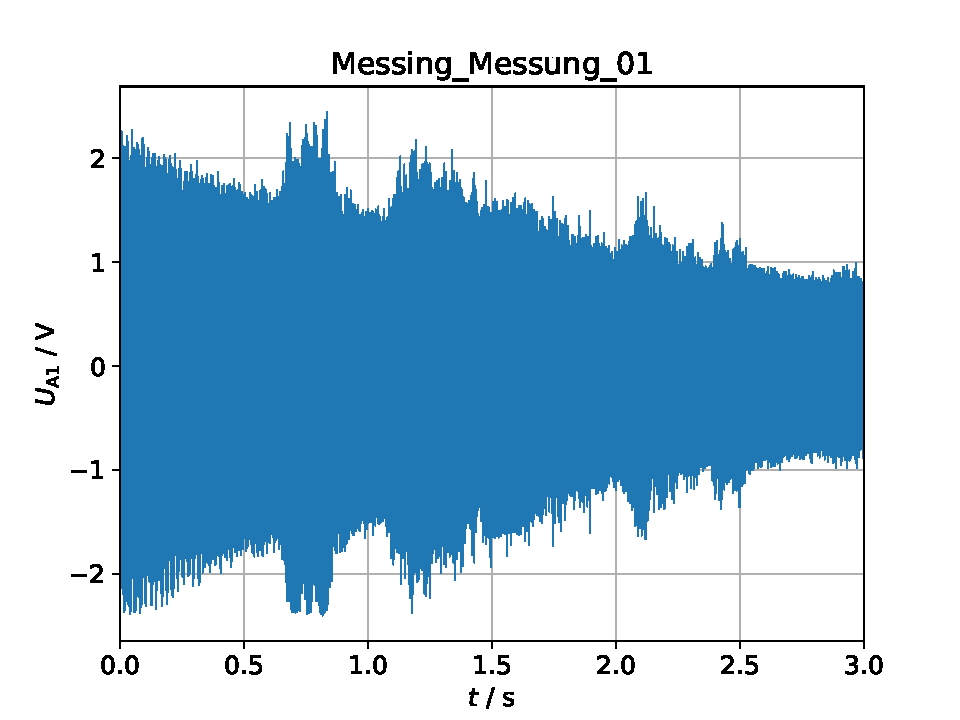
\includegraphics[width=0.5\textwidth]{plots/434170_428396_1A3_Messing_Messung_01_plot.pdf}}
  \subfloat{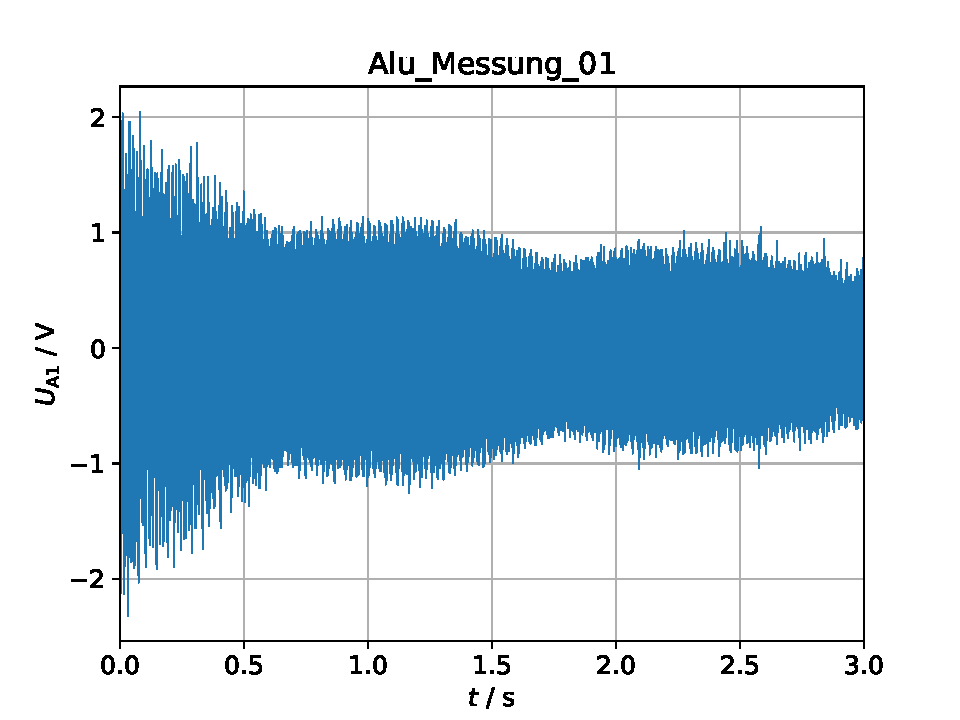
\includegraphics[width=0.5\textwidth]{plots/434170_428396_1A3_Alu_Messung_01_plot.pdf}}
\end{figure}
\begin{figure}[H]
  \centering
  \subfloat{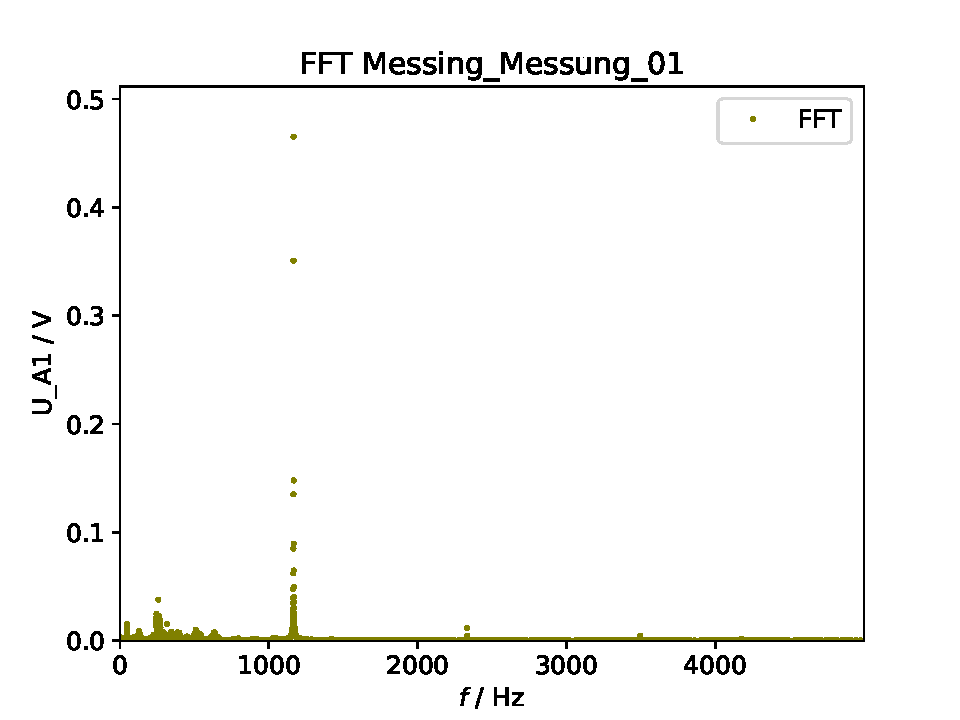
\includegraphics[width=0.5\textwidth]{plots/434170_428396_1A3_Messing_Messung_01_fft.pdf}}
  \subfloat{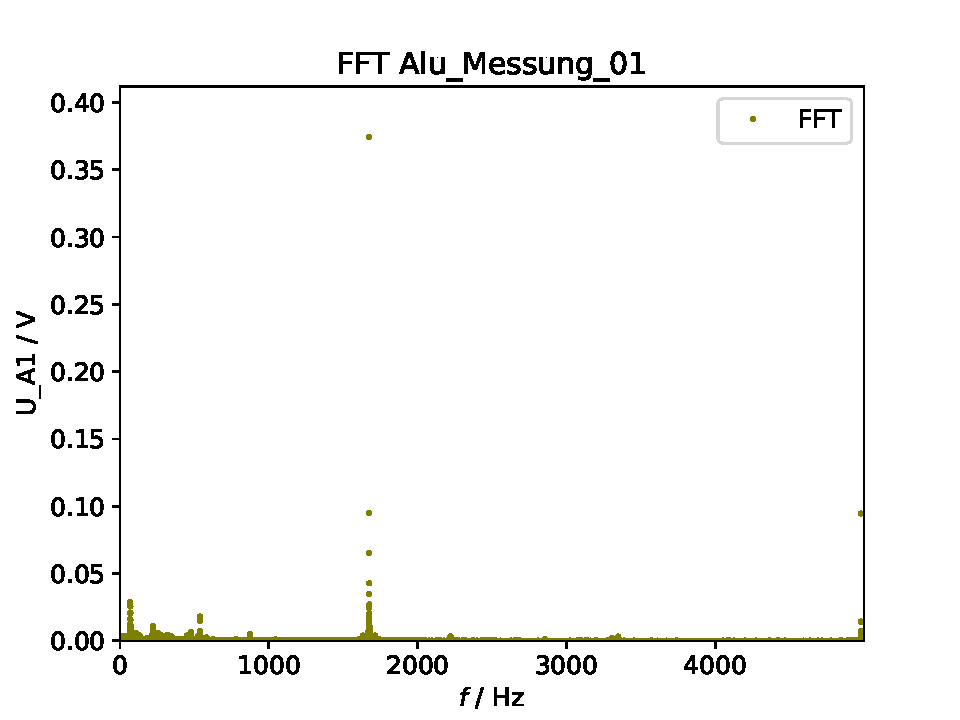
\includegraphics[width=0.5\textwidth]{plots/434170_428396_1A3_Alu_Messung_01_fft.pdf}}
\end{figure}
\begin{figure}[H]
  \centering
  \subfloat{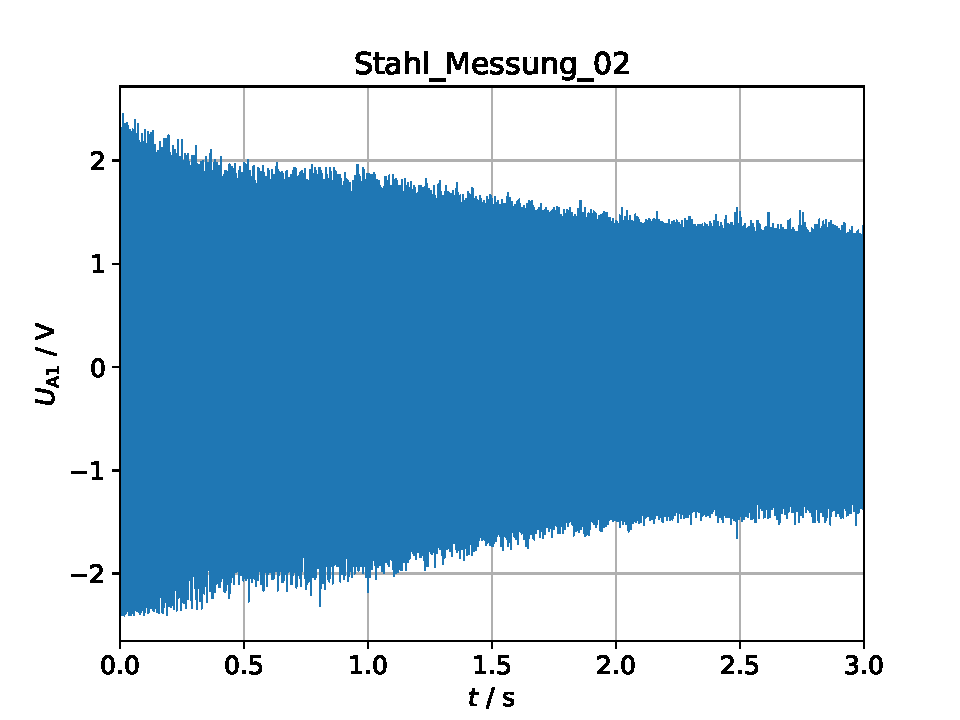
\includegraphics[width=0.5\textwidth]{plots/434170_428396_1A3_Stahl_Messung_02_plot.pdf}}
  \subfloat{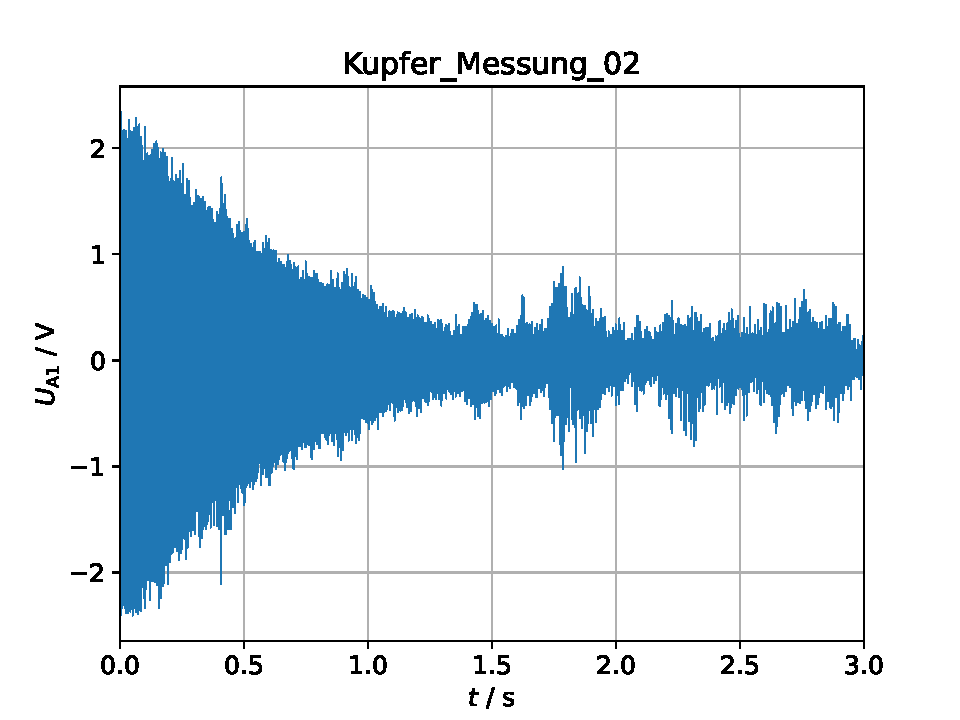
\includegraphics[width=0.5\textwidth]{plots/434170_428396_1A3_Kupfer_Messung_02_plot.pdf}}
\end{figure}
\begin{figure}[H]
  \centering
  \subfloat{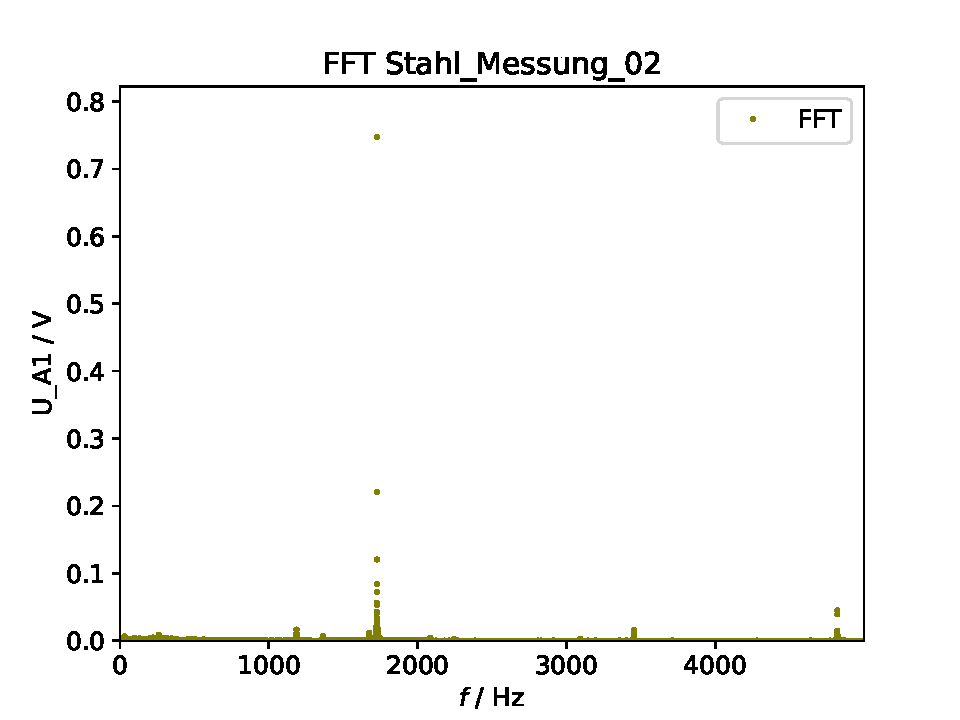
\includegraphics[width=0.5\textwidth]{plots/434170_428396_1A3_Stahl_Messung_02_fft.pdf}}
  \subfloat{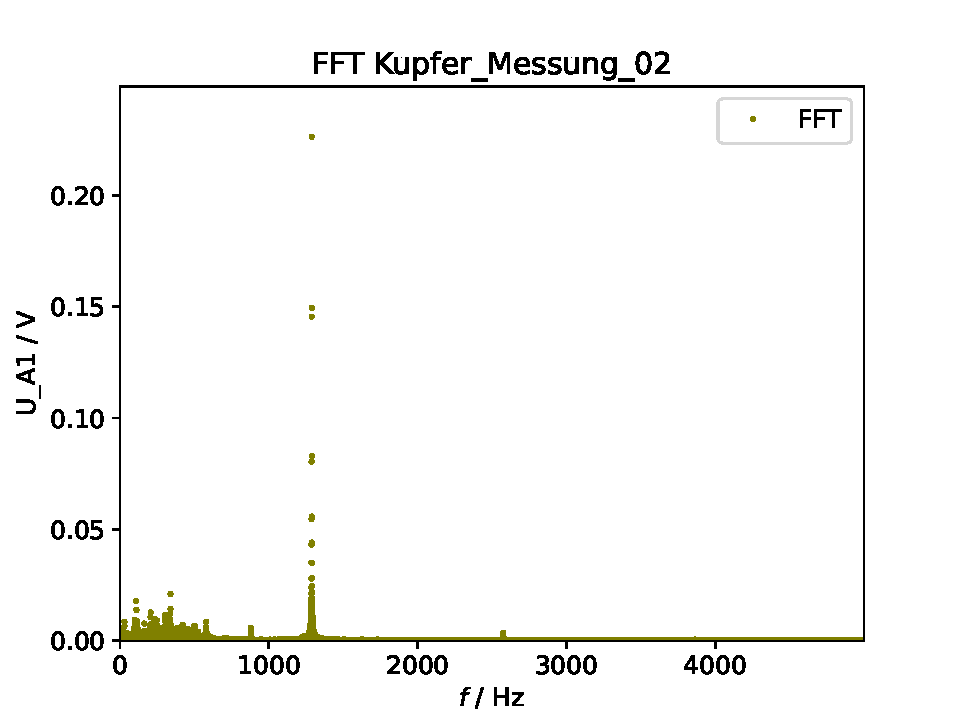
\includegraphics[width=0.5\textwidth]{plots/434170_428396_1A3_Kupfer_Messung_02_fft.pdf}}
\end{figure}

\begin{figure}[H]
    \caption{Exemlpariche Messung mit Störungen und zugehörigen Fouierspektren}
  \centering
    \subfloat[Sättugung vom Mikrophon am Anfang der Messung]{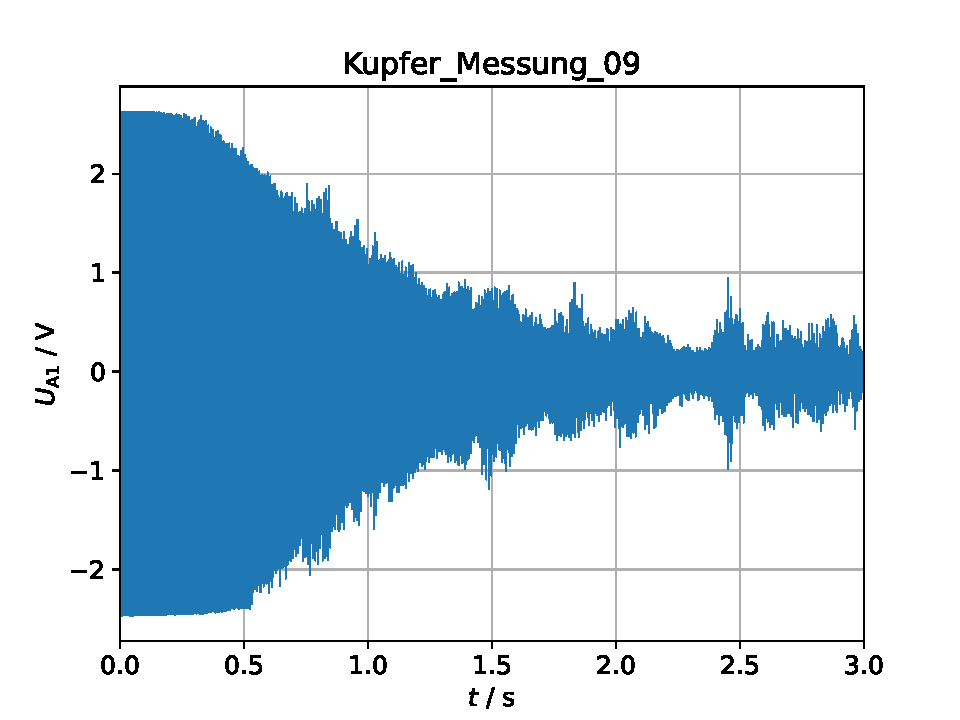
\includegraphics[width=0.5\textwidth]{plots/434170_428396_1A3_Kupfer_Messung_09_plot.pdf}}
    \subfloat[Viele Störgeräusche]{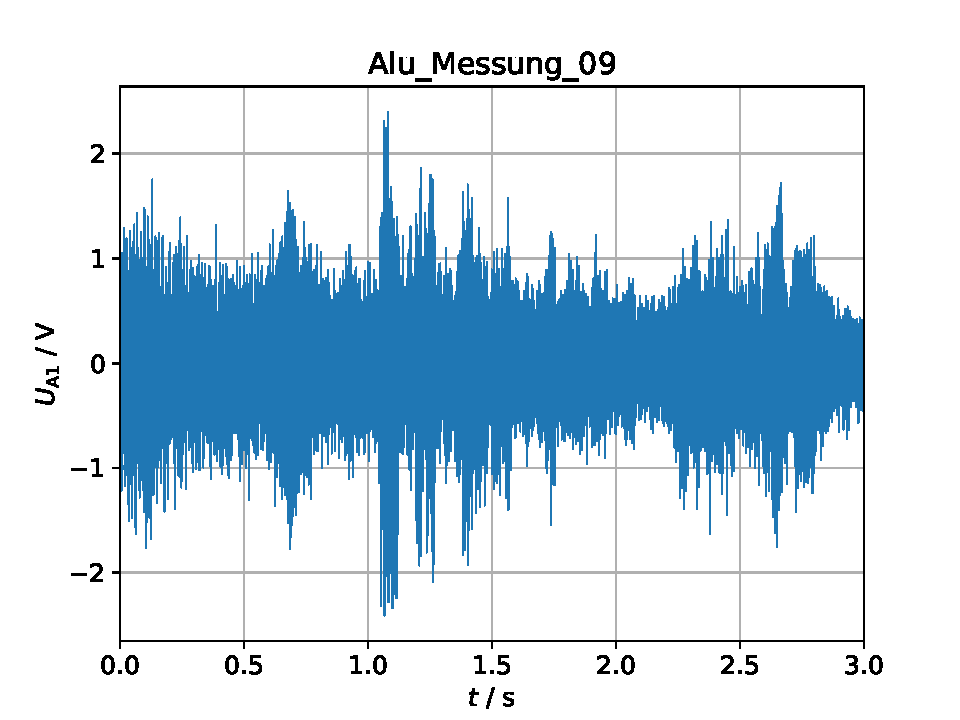
\includegraphics[width=0.5\textwidth]{plots/434170_428396_1A3_Alu_Messung_09_plot.pdf}}
\end{figure}
\begin{figure}[H]
  \centering
    \subfloat{\includegraphics[width=0.5\textwidth]{plots/434170_428396_1A3_Kupfer_Messung_09_fft.pdf}}
    \subfloat{\includegraphics[width=0.5\textwidth]{plots/434170_428396_1A3_Alu_Messung_09_fft.pdf}}
\end{figure}


% schlechte Messungen:
    % Alu Messung 09 (Peak nicht gefunden, viel rauchen)
    % Kupfer einspann Fehler 3 (Peak nicht gefunden, viel rauchen)
    % Kupfer Messung 06 (Uebersteuern)
    % Kufper Einspann Fehler 06 (Peak nicht gefunden, viel rauchen)
    % Alu Messung 04 (Peak nicht gefunden, viel rauchen)
    % Alu Messung 02 (Peak nicht gefunden, viel rauchen)
    % Alu Messung 06 (Peak nicht gefunden, viel rauchen)
    % Stahl Messung 03 (Peak nicht gefunden, viel rauchen)
    % Kupfer Einsann Fehler 04 (Peak nicht gefunden, viel rauchen)
    % Alu Messung 07 (Peak nicht gefunden, viel rauchen)
    % kupfer Messung 10 (Peak nicht gefunden, viel rauchen)
    % Kupfer einsann fehler 05 (Peak nicht gefunden, viel rauchen)
    % Alu Messung 03 (Peak nicht gefunden, viel rauchen)
    % Alu Messung 05 (Peak nicht gefunden, viel rauchen)


% Gute Messung
    % Stahl Test 01
    % Stahl Messung 08
    % Kupfer Messung 01 (Gute abfall, man sieht störgeräusche) (Peak nicht gefunden)
    % Kupfer Einspann Fehler (Man sieht die abnahme gut)
    % Kupfer Test (Man sieht die abnahme gut)


% zu löschende Messungen:
    % Kupfer Einspann Fehler 05

% Graph von schlechter Messung, 
\end{aufgabe}

\begin{aufgabe}{Auswertung}

\textbf{aufarbeitung Rohdaten}\\

    
    Zunächst haben wir unsere gemessenen Daten der Schwingung aufbereitet und selektiert.
    Dies ist sinnvoll, da es verschiedene Fehlerquellen gibt (Störgeräusche, unsaubere Messung, übersteuerung, etc.) die das Ergebniss verfälschen können.
    Diese Fehlerquellen können einen signifikanten einfluss auf das Endgültige Ergebniss haben.
    Um diesen Einfluss möglichst gering zu halten, sollten deshalb die Rohdaten alle angeschaut und aufbereitet werden.
    Hierbei muss auf verschiedene Dinge geachtet werden.
    Diese werden im Folgenden an Beispielen Diskutiert. 

%TODO : Einfügen einer Grafik in der man viele Störgeräusche sieht. 

\begin{figure}[H]
    \caption{Eine Messung mit vielen Störgeräuschen, und trotzem guter Fourieranalyse}
  \centering
    \subfloat{\includegraphics[width=0.5\textwidth]{plots/434170_428396_1A3_Alu_Messung_07_plot.pdf}}
    \subfloat{\includegraphics[width=0.5\textwidth]{plots/434170_428396_1A3_Alu_Messung_07_fft.pdf}}
\end{figure}
 
Oben können sie einen Exemplarischen Graphen von einer Messung sehen, bei der es viele Störgeräusche gab.
Wenn wir uns nun jedoch das Frequenzspektrum anschauen, können wir diese Störgeräusche klar von der Frequenz des Stabes unterscheiden.
Im Frequenzbereich des Stabes, sind keine störenden Geräusche, weswegen bei diesen Messdaten keine Datenpunkte entfernt werden müssen zur erhöhung der Genauheit.
Dies gilt auch für alle weiteren Messungen in welchen Störgeräusche vorhanden waren. 

Bei einigen Messungen wurde der Stab anfangs zu stark angeschlagen, weswegen die Gemessene Amplitude anfangs im gesättigten Bereich liegt.
Da dies die gemessene Grundfrequenz beeeinflussen kann  haben wir bei diesen Messungen die Daten bis zu dem Punkt, wo die Amplitude unter 2.5V ist, weg geschnitten.
Dies verfälscht das Ergebnis nicht, da es nur ein kleines Intervall ist, und wir somit trotzdem Datenpunkte von mehr als 2.5s Messung haben.
Dies ist ein ausreichend großes Intervall.\\
In der Durchführung wurde bereits diskutiert, dass wir Messintervalle von 100$\mu$s verwenden können und damit eine ausreichende Abtastrate haben.
Somit werden auch in einem Intervall von 2.5s  genügend Messpunkte aufgenommen, um daraus die Frequenz ermitteln zu können.

\begin{figure}[H]
  \centering
  \caption{Messung ohne weggeschnittenem Anfang}
  \subfloat{\includegraphics[width=0.5\textwidth]{plots/434170_428396_1A3__Kupfer_Einsp_Fehler_01_plot.pdf}}
  \hfill
  \subfloat{\includegraphics[width=0.5\textwidth]{plots/434170_428396_1A3__Kupfer_Einsp_Fehler_01_fft.pdf}}
\end{figure}

\begin{figure}[H]
  \centering
  \caption{Messung mit weggeschnittenem Anfang}
  \subfloat{\includegraphics[width=0.5\textwidth]{plots/434170_428396_1A3_Kupfer_Einsp_Fehler_01_plot.pdf}}
  \hfill
  \subfloat{\includegraphics[width=0.5\textwidth]{plots/434170_428396_1A3_Kupfer_Einsp_Fehler_01_fft.pdf}}
\end{figure}

%TODO : Einfügen der Grafiken für den Abgeschnittenen und nicht abgeschnittenen Bereich

Oben können sie einen Exemplarischen Graphen von unserer Messung: Kupfer\_Einsp\_Fehler\_01 sehen, in welchem man sehr gut sehen kann, dass anfangs die Amplitude im gesättigten Bereich war, und somit auch nichts über 2.5V aufgezeichnet wurde.
In dieser Messung haben wir also 0.5s weggeschnitten damit der mögliche Effekt davon keinen Einfluss auf unser Ergebnis haben.
Sie können auch die FFT dieser Messung sehen, und den daraus berechneten Peak.
Wobei wir bei der FFT nur dem Relevanten Bereich zwischen 0 und 2000 Hz dargestellt haben.
An dem Wert des Peaks können Sie sehen, dass das Wegschneiden des Anfangs einen Einfluss hatte.
Dieser tritt jedoch erst in der zweiten Nachkommastelle auf.
Ist also ein geringer Einfluss.
Wir wollen ihn jedoch der Genauheithalber nicht vernachlässigen.
Und schneiden somit bei den Messdaten bei denen anfangs übersteuert wurde einen Teil ab. 


Eine genaue Auflistung von allen Daten bei denen wir den Anfang oder das Ende weggeschnitten haben, zur bestimmung der Frequenz wird unten angegeben.
Dieses hier ist nur eine Exemplarische Diskussion warum dies sinnvoll ist.

Wir hatten bei unserer Messreihe 5. eine Messung (Kupfer\_einsp\_Fehler\_05) bei welcher auf Grund von Störgeräuschen und anderen Messeinflüssen wir ein sehr unsauberes Frequenzspektrum nach der Fouieranalyse erhalten haben.
\begin{figure}[H]
  \centering
    \caption{Messung mit sehr starken Störungen auch über 1000 Hz}
  \subfloat{\includegraphics[width=0.5\textwidth]{plots/434170_428396_1A3_Kupfer_Einsp_Fehler_05_plot.pdf}}
  \hfill
  \subfloat{\includegraphics[width=0.5\textwidth]{plots/434170_428396_1A3_Kupfer_Einsp_Fehler_05_fft.pdf}}
\end{figure}

In der FFT kann man sehr gut erkennen, dass wir auch eine vergleichsweise starke Streuung der Frequenzen im Bereich der zu Ermittelnden Grundfrequenz haben.
Aufgrund der ungenauen Messung haben wir sie nicht bei der Auswertung berücksichtigt.
Diese ist aber die einzige Messung, welche wir nicht berücksichtigt haben. \\
 

\textbf{Liste der Messungen bei denen Teile weggeschnitten wurden:}
\begin{itemize}
\item Alu\_Messung\_8 bis 0.45s
\item Kupfer\_Einsp\_Fehler\_1 bis 0.5s
\item Kupfer\_Einsp\_Fehler\_5 ab 2s EVLT LOESCHEN
\item Kupfer\_Einsp\_Fehler\_6 ab 2s
\item Kupfer\_Messung\_1 ab 2.75s
\item Kupfer\_Messung\_3 bis 0.5s
\item Kupfer\_Messung\_4 bis 0.5s
\item Kupfer\_Messung\_6 bis 0.5s
\item Kupfer\_Messung\_7 bis 0.5s
\item Kupfer\_Messung\_9 bis 0.5s
\item Messing\_Messung\_6 bis 0.5s
\item Messing\_Messung\_7 bis 0.5s
\item Stahl\_Messung\_1 bis 0.2s
\item Stahl\_Messung\_9 bis 0.5s
\end{itemize}
% TODO kupfer testmessung mit messung 1 austauschen

\textbf{Systematischer Fehler}\\

Für die Auswertung der Daten und der Entgültigen Berechnung der Elastizitätsmoduls, müssen wir die Fehler 
auf folgende Größen beachten. 
Hier sind sowohl die Statistischen Fehler als auch die Systematischen Fehler relevant.\\


\textbf{Fehlerbehaftete Größen:}
\begin{itemize}
\item Länge der Metallstangen (Systematischer Fehler)
\item Masse der Metallstangen (Systematisher Fehler)
\item Durchmesser der Metallstangen (Systematischer und Statistischer Fehler)
\item Gemessene Schwingungsfrequenz (Systematischer und Statistischer Fehler)
\end{itemize}

Zunächst ein mal die Systematischen Fehler, diese müssen getrennt von den Statistischen Fehlern fortgeplanzt werden. Wir haben einen Systematischen Fehler auf alle unsere Messgrößen. Bei der Längenmessung rürt dies von der Genauigkeit des Bandmaß, dies hängt von der Güteklasse des Bandmaß ab. In unserem Fall haben wir die Güteklasse II. Bei der Analysewage  hängt dieser auch von der Genauigkeit ab, so wie bei der Mikrometerschraube. 
Diese Informationen werden vom Hersteller gegeben, und können im Datenblatt des Geräts nachgeschlagen werden. 

%TODO : Formelzeichen besser übersichtlich darstellen

Der Systematische Fehler bei der Frequenz kommt durch die Digitalisierung des akustischen Signals. Hierfür ist die verwendete Spannungsintervallbreite und die Auflösung (12Bit) relevant. Daraus berechnet sich der Systematische Fehler folgendermaßen. Wobei  $\mathbf{\sigma_fs}$ der Systematische Fehler auf die Frequenz ist, \textbf{I} die Spannungsintervallbreite (Da wir einen Bereich von -3V bis 3V gewählt haben) und \textbf{A} die Auflösung. Im Folgenden bezeichnen ein $\sigma_i$ mit einem Index immer einen Fehler auf eine Messgröße. 
\begin{equation}
         a = \frac{I}{A}
    \end{equation}
\begin{equation}
         \Rightarrow 
         \sigma_fs = \frac{a}{\sqrt{12}}
\end{equation}

Zusätzlich zu diesem Systematischen Fehler, erhalten wir noch einen Systematischen Fehler durch den Einfluss der Einspannposition. Diesen schätzen wir mithilfe unserer Messreihe Kuper\_Einspann\_Fehler ab.  

Somit kennen wir die Systematischen Fehler auf alle unsere Größen.\\

%TODO : Systematischer Fehler auf Frequenz bestimmen

Tabelle der Systematischen Fehler auf einzelne Messgrößen: 

 \begin{table}[H]
        \centering
        \begin{tabularx}{0.8\textwidth}{X l} % adjust width as needed
            \toprule
            \textbf{Metall Stange} & \textbf{Masse} \\
            \midrule
            Masse & $\pm$0.2g \\
            Länge & $\pm$0.7mm\\
            Durchmesser & $\pm$0.01mm \\
            Frequenz & $\pm$0.423mV (Digitalisierung)\\
            & $\pm$0.000000mV\\
            \bottomrule
        \end{tabularx}
        \label{tab:mytable}
    \end{table}

\textbf{auswertung der Schwingungsmessungen}\\


%TODO : Einfügen der Tabelle in der alle Frequenzen der Materialien aufgelistet sind


Aus underen Messreihen 1 bis 4 konten wir mithilfe einer FFT die wir mit Python durchgeführt haben die Grundfrequenz bestimmen.
Hierführ haben wir das Lokale Maximum im Intervall 1000 bis 2000 Herz ermittelt, um Umgebungsrauschen nicht zu berücksichtigen.
Da wir für Metalle erwarten, dass die Schwingungsfrequenz in diesem Bereich liegt, und eine analyse der Rohdaten dieses auch für alle Messungen bestätigt hat, können wir dieses verlustfrei machen.
So konnte auch sichergestellt werden, dass wir nicht die Peaks von Störgeräuschen (Reden, andere Stangen, etc.) ermitteln.
In der Folgenden Tabelle werden unsere Ergebnisse für die Frequenzen der einzelnen Stangen dargestellt.


 \begin{table}[H]
        \centering
        \begin{tabularx}{1.00\textwidth}{X X X X X} % adjust width as needed
            \toprule
            \textbf{Messung Nr.} & \textbf{Stahl 15} & \textbf{Aluminium} & \textbf{Messing} & \textbf{Kupfer} \\
            \midrule
             
                Nr. 1 & 1726.73Hz & 1673.88Hz & 1166.31Hz & 1288.93Hz \\
                Nr. 2 & 1726.02Hz & 1673.85Hz & 1166.53Hz & 1288.11Hz \\
                Nr. 3 & 1726.21Hz & 1673.61Hz & 1166.28Hz & 1288.03Hz \\
                Nr. 4 & 1726.45Hz & 1673.73Hz & 1166.32Hz & 1288.15Hz \\
                Nr. 5 & 1726.29Hz & 1673.67Hz & 1166.27Hz & 1287.99Hz \\
                Nr. 6 & 1726.41Hz & 1673.81Hz & 1166.47Hz & 1288.03Hz \\
                Nr. 7 & 1726.64Hz & 1673.02Hz & 1166.29Hz & 1288.02Hz \\
                Nr. 8 & 1726.76Hz & 1673.52Hz & 1166.32Hz & 1288.13Hz \\
                Nr. 9 & 1726.90Hz & 1671.98Hz & 1166.41Hz & 1288.13Hz \\
                Nr. 10 & 1726.88Hz & 1673.6Hz & 1166.79Hz & 1288.66Hz \\
                 
            \bottomrule
        \end{tabularx}
        \label{tab:mytable}
    \end{table}
    


Aus den oben angeführten Frequen haben wir dann mit Hilfe eines Pyton program (Mat1Mat2Statistik) das Arythmetische mittel und daraus den Resultierenden statistischen Fehler berechnet. Hierfür haben wir folgende Beziehungen für Statistische Messunsicherheiten verwendet. Wobei $\mu$ im allgemeinen der Mittelwert ist, $s^2$ die Varianz und $\sigma_i$ der fehler auf die Größe ist.

\begin{equation}
	\mu = \frac{1}{n}\sum_{i=1}^nx_i
\end{equation}

\begin{equation}
	s^2 = \frac{1}{n-1}\sum_{i=1}^n(\mu-x_i)^2
\end{equation}

\begin{equation}
	\sigma_f = \frac{s}{\sqrt{n}} 
\end{equation}

Für die verschiedenen Stangen ergaben sich dann Folgende Mittelwerte und statistische Fehler.\\


 \begin{table}[H]
        \centering
        \begin{tabularx}{0.8\textwidth}{X X X} % adjust width as needed
            \toprule
            \textbf{Metall Stange} & \textbf{Erwartungs Wert} & \textbf{Standardabweichung} \\
            \midrule
            Stahl 15 & 1726.53Hz & $\pm$0.094Hz \\
            Aluminium & 1673.47Hz & $\pm$0.18Hz \\
            Messing & 1166.40Hz & $\pm$0.052Hz \\
            Kupfer & 1288.22Hz & $\pm$0.10Hz \\

            \bottomrule
        \end{tabularx}
        \label{tab:mytable}
    \end{table}
    
Als weiteren Statistischen Fehler haben wer den Fehler der bei der mehrfachen Messung des Durchmessers der Stangen auftritt.
Wir haben diese mehrfach gemessen, um zu überprüfen ob unsere Annahme, dass die Stange einen 
Kreisförmigen Querschnitt hat gerechtfertigt ist. Zur bestimmung des Mittelwerts und Fehlers auf den Durchmesser 
haben wir ebenfalls das Pythonprogramm ... benutzt. 
Daraus ergibt sich:\\

 \begin{table}[H]
        \centering
        \begin{tabularx}{0.8\textwidth}{X c c} % adjust width as needed
            \toprule
            \textbf{Metall Stange} & \textbf{Erwartungs Wert} & \textbf{Standardabweichung} \\
            \midrule
            Stahl 15 & 12.000mm & $\pm$0.001mm \\
            Aluminium & 12.057mm & $\pm$0.002mm  \\
            Messing & 11.986mm & $\pm$0.003mm \\
            Kuper & 11.981mm & $\pm$0.001mm \\
            \bottomrule
        \end{tabularx}
        \label{tab:mytable}
    \end{table}

Somit haben wir den Messfehler auf alle Größen bestimmt und können damit das elastizitätsmodul berechnen. Hierbei müssen die Statistischen und die Systematischen Fehler getrennt fortgeplanzt werden.

Für die Fehlerfortplanzung der Statistischen Fehler gilt: (hier wir die Gaußsche fehlerfortplanzung verwendet) 

\begin{equation}
	\sigma_y^2 = \sum_{i,j=1}^n\left[\frac{\partial y}{\partial x_i}\frac{\partial y}{\partial x_j}\right]_{x=\mu}V_{ij}^2
\end{equation}
Hier steht $V_{ij}$ für die Varianz zwischen denn Variablen. In unserem Fall sind die Variablendie Masse, Länge, Grundfrequenz und Durchmesser. 
Bei diesen können wir davon ausgehen, dass diese Größen unkorreliert sind. 
Also unsere Längenmessung keinen Einfluss auf die Messung des Durchmessers und der Masse hatte.
Das selbe gilt für die anderen Messgrößen. 
Somit müssen wir den Mischterm auf Grund der Covarianz nicht beachten da diese null ist.
Somit vereinfacht sich die Gauß'sche Fehlerfortplanzung zu:

\begin{equation}
	\sigma_y^2 = \sum_{i=1}^n\left[\frac{\partial y}{\partial x_i}\right]_{x=\mu}\sigma_{i}^2
\end{equation}

Bei den Systematischen Fehlern verwenden wir die Methode der Größtfehlerabschätzung. 
Dies ist zwar eine sehr konservative schätzung des Fehlers, in diesem Fall jedoch sinnvoll,
da Masse und Länge je nur einmal gemessen wurden. wenn nun $\Delta x_1$, $\Delta x_2$, $\Delta x_3$
die eingehenden Einzelfehler sind, ist die lineare Fehlerfortplanzung: \\

\begin{equation}
	\Delta y = \left|\frac{\partial y}{\partial x_1}\Delta x_1\right| + 
	\left|\frac{\partial y}{\partial x_2}\Delta x_2\right| + 
	\left|\frac{\partial y}{\partial x_3}\Delta x_3\right|
\end{equation}\\


Als Zwischenergebnis berechnen wir zuerst die Dichte. Hierführ berechnen wir den
Erwartungswert der Dichte indem wir die Mittlewerte der Benötigten größen Verwenden. 
Wir verwenden die Formel die in dem Abschnitt Grundlagen eingeführt werden. Die Rechnung haben wir mit Python durchgeführt. Diese können sie in der Datei ... nachlesen.\\

\begin{equation}
	formel\quad zur \quad berechnung \quad der \quad Dichte: \qquad \rho = \frac{M}{V} = \frac{4M}{\pi D^2L}
\end{equation}

\end{aufgabe}
%TODO : Argumentation warum die Fehler unkoreliert sind
%TODO : Elastizitätsmodul berechnen
%TODO : Fehlerfortplanzung E-Modul
%TODO : Fehlerfortplanzung Dichte
%TODO : Darstellung der Frequenzen in Plot und err von systematisch
%TODO : E-Modul in Plot
%TODO : Vergleichen mit Literaturwerten
%TODO : Diskussioon der Fehlerbeiträge, was dominiert den Gesamtfehler
%TODO : Statistische messungenauigkeit auf L & M 
%TODO : Vergleich mit Literaturwerten
%TODO : Statistische Fehler mit Sigma Systematische mit Delta
%TODO : Dichte bei Grundlagen hinzufügen
%TODO : Gesamtprotokoll auf Konsistenz überprüfen in Bezeichnung 
%TODO : Programme übersichtlich machen und kommentieren
\end{document}